\documentclass[aspectratio=169,10pt]{beamer}
\usetheme{Simple}

\usepackage[UTF8,fontset=fandol]{ctex}
\usepackage{amsmath,amssymb,booktabs,array,tabularx,multirow}
\usepackage{graphicx,xcolor,xurl,hyperref}
\usepackage{tikz}
\usetikzlibrary{arrows.meta,calc,fit,positioning,shapes.geometric}

\graphicspath{{Figures/}{experiments/sglsim_large/traces/cc-traces-weka-062126/analysis/workflow_examples/}}
\setbeamertemplate{caption}[numbered]
\setbeamertemplate{equation number}[numbered]
\setbeamertemplate{navigation symbols}{}

\definecolor{AegisBlue}{RGB}{38,91,145}
\definecolor{AegisBlueLight}{RGB}{232,242,251}
\definecolor{AegisOrange}{RGB}{188,112,38}
\definecolor{AegisOrangeLight}{RGB}{255,241,224}
\definecolor{AegisGreen}{RGB}{41,126,91}
\definecolor{AegisGreenLight}{RGB}{226,245,236}
\definecolor{AegisPurple}{RGB}{104,78,157}
\definecolor{AegisPurpleLight}{RGB}{242,238,250}
\definecolor{AegisRed}{RGB}{181,66,61}
\definecolor{AegisRedLight}{RGB}{252,232,230}
\definecolor{AegisGray}{RGB}{77,87,99}
\definecolor{AegisGrayLight}{RGB}{246,247,249}

\newcommand{\AegisKV}{AegisKV}
\newcommand{\code}[1]{\texttt{\footnotesize #1}}
\newcommand{\tightitems}{\setlength{\itemsep}{2pt}\setlength{\parskip}{0pt}}
\newcommand{\boundary}[1]{%
  \begin{beamercolorbox}[rounded=true,sep=0.75ex,wd=0.98\textwidth]{block body}
    \scriptsize\textbf{边界：}#1
  \end{beamercolorbox}}
\newcommand{\takeaway}[1]{%
  \begin{beamercolorbox}[rounded=true,sep=0.75ex,wd=0.98\textwidth]{block body}
    \footnotesize\textbf{结论：}#1
  \end{beamercolorbox}}
\newcommand{\layercard}[3]{%
  \begin{beamercolorbox}[wd=\textwidth,rounded=true,sep=0.9ex]{block body}
    {\color{#1}\textbf{#2}}\par\vspace{0.3ex}\scriptsize #3
  \end{beamercolorbox}}

\newcounter{paperalgline}
\newenvironment{paperalgo}[1]{%
  \setcounter{paperalgline}{0}
  \begin{minipage}{\textwidth}
  \hrule height 0.5pt\vspace{0.3ex}
  {\footnotesize\textbf{#1}\par}\vspace{0.2ex}\hrule height 0.35pt\vspace{0.35ex}
  \scriptsize\begin{tabular}{@{}r@{\hspace{0.45em}}p{0.88\textwidth}@{}}
}{%
  \end{tabular}\vspace{0.3ex}\hrule height 0.5pt
  \end{minipage}
}
\newcommand{\algline}[1]{\stepcounter{paperalgline}\arabic{paperalgline}: & #1 \\}

\def\meetingname{AegisKV Complete System Design}
\title{\AegisKV{}：面向 Agent Workflow 的 Slack-Aware KV 恢复系统}
\subtitle{Workflow Slack · Recovery Placement · L1/L2 Backup Right-Sizing}
\author[Zhao]{Zhan Zhao}
\institute[HKBU]{Hong Kong Baptist University}
\date[2026.07.20]{\meetingname\\2026 年 7 月 20 日}

\hfuzz=20pt
\hbadness=10000
\vfuzz=20pt
\vbadness=10000
\emergencystretch=2em

% Keep the deck compact: section titles appear in the outline, but do not
% consume a standalone transition page.
\AtBeginSection[]{}

\begin{document}

\begin{frame}[plain]
  \titlepage
\end{frame}

% !TeX root = ../paper_outline.tex
\section{问题与系统总览}

\begin{frame}{AegisKV | 系统目标：用有限备份资源降低工作流故障延迟}
  \small
  智能体工作流的完成时间由依赖路径决定。worker/GPU 故障后，KV 恢复只有在
  恢复延迟超过请求松弛时间时才增加工作流完成时间：
  \begin{equation}
    \begin{aligned}
      \operatorname{WCT}_w
      &=\operatorname{WCT}_w^{0}
        +\Delta\operatorname{WCT}_w^{\mathrm{fail}},\\
      (\mathbf x^{(k)},\mathbf D^{(k)})
      &=\mathcal P(
        \widehat{\boldsymbol\sigma},\text{KV 块},\text{恢复路径};
        \boldsymbol\alpha^{(k)},\boldsymbol\beta^{(k)}),\\
      (\boldsymbol\alpha^{(k+1)},\boldsymbol\beta^{(k+1)})
      &=\mathcal C(
        \mathbf L_1^{(k)},\mathbf L_2^{(k)},
        \mathbf D_1^{(k)},\mathbf D_2^{(k)}).
    \end{aligned}
    \label{eq:system-objective}
  \end{equation}

  \scriptsize
  $\operatorname{WCT}_w^{0}$ 是无故障完成时间；
  $\Delta\operatorname{WCT}_w^{\mathrm{fail}}$ 是 failure-time recovery 的可见增量；
  $\mathbf x^{(k)}$ 是算法 2 的备份动作，$\mathbf D^{(k)}$ 是容量截断前影子需求；
  $\mathbf L_1^{(k)},\mathbf L_2^{(k)}$ 是逐节点正常负载；
  $\boldsymbol\alpha,\boldsymbol\beta$ 分别是 L1 HBM 与 L2 Host DRAM 的备份比例。
  算法 2 在窗口 $k$ 使用当前预算，算法 3 用其反馈确定窗口 $k+1$ 的预算。
  系统受三类硬约束限制：

  \vspace{0.07cm}
  \renewcommand{\arraystretch}{1.17}
  \begin{tabularx}{\textwidth}{p{0.20\textwidth}X}
    \toprule
    约束 & 系统含义 \\
    \midrule
    Correctness & 只恢复 committed、version-valid、跨故障域的 KV chunk \\
    Normal-path SLO & backup copy 与 L1/L2 reservation 不得突破 no-failure p99/OOM 上限 \\
    Capacity & L1 HBM 与 L2 Host DRAM 都使用显式 per-node backup ratio \\
    \bottomrule
  \end{tabularx}

  \vspace{0.08cm}
  \takeaway{算法 2 负责容量约束下的备份决策；算法 3 根据正常负载和算法 2
  的本窗口需求反馈，确定下一窗口的 $\alpha_n,\beta_n$。}
\end{frame}

\begin{frame}{AegisKV | 完整架构：三个控制算法与一个恢复数据面}
  \centering
  \begin{tikzpicture}[
    x=1cm,y=1cm,
    box/.style={draw,rounded corners=2pt,align=center,font=\scriptsize,
                minimum height=0.78cm,inner sep=5pt},
    app/.style={box,draw=AegisBlue,fill=AegisBlueLight,minimum width=2.10cm},
    route/.style={box,draw=AegisPurple,fill=AegisPurpleLight,minimum width=2.55cm},
    algtwo/.style={box,draw=AegisOrange,fill=AegisOrangeLight,minimum width=2.15cm},
    algthree/.style={box,draw=AegisGreen,fill=AegisGreenLight,minimum width=2.15cm},
    data/.style={box,draw=AegisGray,fill=AegisGrayLight,minimum width=2.15cm},
    arr/.style={-{Stealth[length=1.8mm]},thick,draw=AegisGray},
    control/.style={-{Stealth[length=1.6mm]},thin,dashed,draw=AegisPurple}
  ]
    \node[app] (alg1) at (0.8,1.3) {算法 1\\DAG 松弛时间};
    \node[route] (router) at (4.0,1.3)
      {Cache-Aware Router\\负载 + Radix Tree\\$\pi_1$: 执行，$\pi_2$: 备份};

    \node[draw=AegisGray,rounded corners=4pt,minimum width=5.7cm,
      minimum height=2.85cm,fill=AegisGrayLight] (dp) at (9.2,1.05) {};
    \node[font=\scriptsize\bfseries,anchor=west] at (6.55,2.25)
      {每个 DP rank：算法与 ACK 权威状态均在本地};
    \node[algtwo] (alg2) at (7.9,1.35) {算法 2\\KV 块 L1/L2/R};
    \node[algthree] (alg3) at (10.5,1.35) {算法 3\\本地 $\alpha/\beta$};
    \node[data,minimum width=4.65cm] (stores) at (9.2,0.15)
      {Backup Manager：复制、ACK、$D/U/O$、Recovery Hint};

    \draw[arr] (alg1) -- node[above,font=\tiny]{请求 + slack} (router);
    \draw[arr] (router) -- node[above,font=\tiny]{$e(r),b(r)$} (alg2);
    \draw[control] (alg3) -- node[above,font=\tiny]{当前预算} (alg2);
    \draw[arr] (alg2) -- (stores);
    \draw[control] (stores.east) to[bend right=20]
      node[right,font=\tiny]{$D/U/O$} (alg3.south);
    \draw[control] (stores.west) to[bend left=24]
      node[below,font=\tiny]{聚合 Recovery Hint} (router.south);
  \end{tikzpicture}

  \vspace{0.14cm}
  \scriptsize
  \renewcommand{\arraystretch}{1.12}
  \begin{tabularx}{\textwidth}{p{0.15\textwidth}p{0.23\textwidth}p{0.27\textwidth}X}
    \toprule
    算法 & 输入 & 发布结果 & 所在层 \\
    \midrule
    算法 1 & 固定工作流 DAG + 时长分布 & 请求松弛时间 & 应用层 \\
    Router 策略 & 正常负载 + Radix Tree & 执行/备份 Rank 绑定 + Retry Rank & Router \\
    算法 2 & 固定 Backup Rank + slack + KV 块 + 当前预算 & L1/L2/R plan + ACK + $D/U/O$ & DP rank \\
    算法 3 & 本地正常负载 + 本地算法 2 反馈 & 下一窗口 $\alpha_n,\beta_n$ & DP rank \\
    \bottomrule
  \end{tabularx}
\end{frame}

\begin{frame}{AegisKV | 跨窗口备份决策闭环}
  \centering
  \begin{tikzpicture}[
    x=1cm,y=1cm,
    event/.style={draw,rounded corners=2pt,align=center,font=\tiny,
                  minimum width=1.62cm,minimum height=0.68cm,inner sep=2pt},
    arr/.style={-{Stealth[length=1.8mm]},thick,draw=AegisGray},
    feedback/.style={-{Stealth[length=1.6mm]},thin,dashed,draw=AegisPurple}
  ]
    \node[event,draw=AegisBlue,fill=AegisBlueLight] (e1) at (0,1.4)
      {1. 固定 DAG\\激活片段};
    \node[event,draw=AegisBlue,fill=AegisBlueLight] (e2) at (2.05,1.4)
      {2. 算法 1\\发布 slack};
    \node[event,draw=AegisPurple,fill=AegisPurpleLight] (e3) at (4.10,1.4)
      {3. Router Top-2\\绑定两个 Rank};
    \node[event,draw=AegisOrange,fill=AegisOrangeLight] (e4) at (6.15,1.4)
      {4. DP 算法 2\\选择 L1/L2/R};
    \node[event,draw=AegisGreen,fill=AegisGreenLight] (e5) at (8.20,1.4)
      {5. 目标 DP\\ACK + Hint};
    \node[event,draw=AegisRed,fill=AegisRedLight] (e6) at (10.25,1.4)
      {6. Failure\\零查询重路由};

    \foreach \a/\b in {e1/e2,e2/e3,e3/e4,e4/e5,e5/e6}
      \draw[arr] (\a) -- (\b);

    \node[event,draw=AegisOrange,fill=AegisOrangeLight,minimum width=2.0cm] (c)
      at (6.15,0) {窗口 $k$ 结束\\发布 $D^{(k)},U^{(k)},O^{(k)}$};
    \node[event,draw=AegisGreen,fill=AegisGreenLight,minimum width=2.0cm] (b)
      at (8.75,0) {算法 3\\发布窗口 $k+1$ 预算};
    \draw[feedback] (e4.south) -- (c.north);
    \draw[arr] (c) -- node[above,font=\tiny]{需求反馈} (b);
    \draw[feedback] (b.north) to[bend right=28]
      node[right,font=\tiny]{下一窗口 $\alpha,\beta$} (e4.south east);
  \end{tikzpicture}

  \vspace{0.18cm}
  \scriptsize
  \begin{columns}[T,onlytextwidth]
    \begin{column}{0.48\textwidth}
      \textbf{Normal path：}
      Router 只给出 $e(r),b(r)$；DP rank 内算法 2 使用当前 $\alpha,\beta$
      决定 KV 层级，算法 3 在窗口边界更新本地预算。
    \end{column}
    \begin{column}{0.48\textwidth}
      \textbf{Failure path：}
      Router 使用已缓存 Recovery Hint、当前负载和 Radix Tree 比较
      Backup Rank 与其他 Rank，不在故障路径发起同步查询。
    \end{column}
  \end{columns}

  \vspace{0.10cm}
  \takeaway{因果链是 $\text{算法 3}(k)\rightarrow\text{算法 2}(k)
  \rightarrow\text{算法 3}(k+1)$，不存在同窗口循环依赖。}

  \vspace{0.05cm}
  \boundary{算法 2/3 与 ACK 权威状态都在 DP rank；Router 只缓存 Recovery Hint 摘要。摘要过期、copy 未 ACK 或版本不匹配时按 Recompute 估价。}
\end{frame}

% !TeX root = ../paper_outline.tex
\section{系统模型}

\begin{frame}{AegisKV | Failure Model 与恢复正确性边界}
  \scriptsize
  \begin{columns}[T,onlytextwidth]
    \begin{column}{0.48\textwidth}
      \begin{block}{Failure model}
        \begin{itemize}
          \tightitems
          \item worker/GPU 发生 crash-stop；owner GPU 的 active KV 全部丢失；
          \item 一次 recovery epoch 处理一个 failure domain；
          \item model weights、request input 与 workflow state 可在 survivor 上获得；
          \item peer GPU/Host 只有位于 owner failure domain 之外才可作为 backup；
          \item detector 发布单调递增的 \code{failure\_epoch}。
        \end{itemize}
      \end{block}
    \end{column}
    \begin{column}{0.48\textwidth}
      \begin{block}{Recovery object}
        \begin{itemize}
          \tightitems
          \item 保护对象是 fixed-size、immutable、committed KV chunk；
          \item 每个 chunk 由 \code{workflow/node/request/span/version} 唯一标识；
          \item mutable decode tail 在 commit frontier 之后，故障时直接 recompute；
          \item 恢复完成后，request 从 verified frontier 继续执行。
        \end{itemize}
      \end{block}
    \end{column}
  \end{columns}

  \vspace{0.10cm}
  \renewcommand{\arraystretch}{1.16}
  \begin{tabularx}{\textwidth}{p{0.12\textwidth}p{0.25\textwidth}X}
    \toprule
    不变量 & 条件 & 保证 \\
    \midrule
    I1 & destination $\notin\operatorname{FD}(\mathrm{owner})$ & owner failure 不同时销毁 backup \\
    I2 & restore version $=$ committed version & 不恢复 stale 或 partial KV \\
    I3 & copy ACK 之前 action 保持 Recompute & 不把 in-flight copy 计为可恢复状态 \\
    I4 & 任一检查失败均回退 Recompute & metadata/copy failure 只损失性能，不损失正确性 \\
    \bottomrule
  \end{tabularx}

  \vspace{0.08cm}
  \takeaway{L1 Backup 与 L2 Backup 是性能优化；Recompute 始终是 correctness-preserving base path。}
\end{frame}

% !TeX root = ../paper_outline.tex
\section{算法 1：工作流松弛时间估计}

\begin{frame}{算法 1 | 工作流示例：多轮节点、扇出/扇入与松弛时间}
  \centering
  \resizebox{0.98\linewidth}{!}{%
  \begin{tikzpicture}[
    x=1cm,y=1cm,
    n/.style={draw=AegisGray,fill=AegisGrayLight,rounded corners=2pt,
              minimum width=2.02cm,minimum height=1.18cm,align=left,
              inner sep=4pt,font=\tiny},
    cp/.style={n,draw=AegisRed,fill=AegisRedLight,very thick},
    arr/.style={-{Stealth[length=1.8mm]},thick,draw=AegisGray},
    cparr/.style={-{Stealth[length=1.8mm]},very thick,draw=AegisRed}
  ]
    \node[cp] (m) at (0,0)
      {\textbf{主规划者}\\T3 委派：1s\\T4 跟进：2s\\\textbf{剩余 3s · 松弛 0s}};

    \node[n] (a) at (3.05,2.0)
      {\textbf{A · 研究者-1}\\T1 搜索：4s\\T2 阅读：3s\\T3 汇总：2s\\\textbf{剩余 9s · 松弛 4s}};
    \node[n] (b) at (3.05,0)
      {\textbf{B · 研究者-2}\\T1 搜索：2s\\T2 验证：4s\\T3 等待：0s\\\textbf{剩余 6s · 松弛 6s}};
    \node[cp] (c) at (3.05,-2.0)
      {\textbf{C · 编码}\\T1 检查：3s\\T2 修改：5s\\T3 测试：4s\\\textbf{剩余 12s · 松弛 0s}};

    \node[n] (d) at (6.15,1.15)
      {\textbf{D · 审阅者}\\T1 审阅：3s\\T2 反馈：2s\\\textbf{剩余 5s · 松弛 4s}};
    \node[cp] (e) at (6.15,-1.15)
      {\textbf{E · 汇总者}\\T1 合并：2s\\T2 修订：4s\\\textbf{剩余 6s · 松弛 0s}};

    \node[cp] (f) at (9.15,0)
      {\textbf{F · 定稿者}\\T1 撰写：2s\\T2 校验：1s\\\textbf{剩余 3s · 松弛 0s}};

    \draw[arr] (m) -- (a);
    \draw[arr] (m) -- (b);
    \draw[cparr] (m) -- (c);
    \draw[arr] (a) -- (d);
    \draw[arr] (b) -- (d);
    \draw[arr] (b) -- (e);
    \draw[cparr] (c) -- (e);
    \draw[arr] (d) -- (f);
    \draw[cparr] (e) -- (f);
  \end{tikzpicture}
  }

  \vspace{0.08cm}
  \scriptsize
  \begin{columns}[T,onlytextwidth]
    \begin{column}{0.48\textwidth}
      \textbf{图中结果：}最长路径为 Main $\rightarrow$ C $\rightarrow$ E $\rightarrow$ F，
      剩余 WCT 为 24s；红色节点的松弛时间为 0。
    \end{column}
    \begin{column}{0.48\textwidth}
      \textbf{运行时更新：}任一轮次完成、执行片段状态或时长分布变化后，
      在同一个固定 DAG 的剩余子图上重新计算关键路径与节点松弛时间。
    \end{column}
  \end{columns}
\end{frame}

% !TeX root = ../paper_outline.tex

\begin{frame}{算法 1 | 两类工作流，一个统一的执行 DAG}
  \small
  任务分解型（Task-decomposition）与角色专门型（Role-specialized）描述不同的
  智能体生命周期和协作语义，但都转换为同一种按时间展开的带属性执行 DAG；
  两者不是互斥分类。

  \vspace{0.08cm}
  \begin{columns}[T,onlytextwidth]
    \begin{column}{0.48\textwidth}
      \centering
      \textbf{任务分解型：临时子智能体执行子任务}

      \vspace{0.05cm}
      \resizebox{0.92\linewidth}{!}{%
      \begin{tikzpicture}[
        n/.style={draw=AegisBlue,fill=AegisBlueLight,rounded corners=2pt,
                  minimum width=1.40cm,minimum height=0.68cm,align=center,font=\scriptsize},
        arr/.style={-{Stealth[length=1.6mm]},thick,draw=AegisGray}
      ]
        \node[n] (m0) at (0,0) {主智能体$^{(0)}$\\委派};
        \node[n] (a) at (2.2,1.05) {子任务 A};
        \node[n] (b) at (2.2,0) {子任务 B};
        \node[n] (c) at (2.2,-1.05) {子任务 C};
        \node[n] (m1) at (4.4,0) {主智能体$^{(1)}$\\汇合};
        \draw[arr] (m0) -- (a);
        \draw[arr] (m0) -- (b);
        \draw[arr] (m0) -- (c);
        \draw[arr] (a) -- (m1);
        \draw[arr] (b) -- (m1);
        \draw[arr] (c) -- (m1);
      \end{tikzpicture}
      }

      \scriptsize
      通常一次短生命周期调用对应一个节点；核心关系是
      \textbf{创建、扇出和汇合（spawn/fan-out/join）}。
    \end{column}
    \begin{column}{0.48\textwidth}
      \centering
      \textbf{角色专门型：持久角色跨阶段复用}

      \vspace{0.05cm}
      \resizebox{0.98\linewidth}{!}{%
      \begin{tikzpicture}[
        n/.style={draw=AegisOrange,fill=AegisOrangeLight,rounded corners=2pt,
                  minimum width=1.32cm,minimum height=0.68cm,align=center,font=\scriptsize},
        arr/.style={-{Stealth[length=1.6mm]},thick,draw=AegisGray}
      ]
        \node[n] (o0) at (0,0) {编排$^{(0)}$};
        \node[n] (r1) at (1.8,0) {研究$^{(1)}$};
        \node[n] (v1) at (3.6,0) {验证$^{(1)}$};
        \node[n] (r2) at (5.4,0) {研究$^{(2)}$};
        \node[n] (o1) at (7.2,0) {编排$^{(1)}$};
        \draw[arr] (o0) -- (r1);
        \draw[arr] (r1) -- (v1);
        \draw[arr] (v1) -- node[above,font=\tiny]{反馈} (r2);
        \draw[arr] (r2) -- (o1);
      \end{tikzpicture}
      }

      \scriptsize
      同一个研究者或编排者可对应多个节点；允许的反馈轮次
      在工作流启动前展开为固定激活片段。
    \end{column}
  \end{columns}

  \vspace{0.12cm}
  \begin{beamercolorbox}[rounded=true,sep=0.75ex,wd=0.98\textwidth]{block body}
    \scriptsize
    \textbf{统一映射：}节点是执行片段（execution episode），不是整个智能体；每个节点
    同时带有智能体、角色、子任务、激活轮次和请求属性。角色协议
    按 $R^{(1)}\!\rightarrow V^{(1)}\!\rightarrow R^{(2)}$ 预先展开，因此执行图固定且无环。
  \end{beamercolorbox}

  \vspace{0.06cm}
  \boundary{Real CC 轨迹直接验证 main/subagent 任务分解型工作流；固定轮次的
  角色专门型 DAG 是统一模型支持的输入形态，仍需带角色标注的轨迹单独验证。}
\end{frame}

\begin{frame}{算法 1 | 固定工作流 DAG 与剩余子图}
  \small
  工作流启动前已知完整 DAG；运行时只根据完成状态取其剩余诱导子图：
  \begin{equation}
    \begin{aligned}
      D_w&=(V_w,E_w),\\
      V_w^{\mathrm{rem}}(t)
        &=\{v\in V_w:\operatorname{status}_v(t)\neq\mathrm{completed}\},\\
      D_w^{\mathrm{rem}}(t)
        &=D_w[V_w^{\mathrm{rem}}(t)].
    \end{aligned}
    \label{eq:fixed-residual-dag}
  \end{equation}

  \scriptsize
  \renewcommand{\arraystretch}{1.14}
  \begin{tabularx}{\textwidth}{p{0.22\textwidth}X}
    \toprule
    规则 & 精确定义 \\
    \midrule
    工作流启动 & 任务/角色适配器在执行前生成全部节点、类型化边与固定轮次 \\
    边语义 & 每条 $e\in E_w$ 都是确定依赖，等价地取 $p_e=1$；不学习边概率 \\
    进度状态 & 节点只在待执行、执行中、已完成之间迁移，不新增分支、节点或边 \\
    剩余子图 & 已完成节点从式~\eqref{eq:fixed-residual-dag} 排除，其后继依赖随之释放 \\
    唯一不确定量 & 待执行或执行中片段的剩余时长 \\
    非研究范围 & 运行中才生成的新分支、无限反馈循环与随机拓扑 \\
    \bottomrule
  \end{tabularx}

  \vspace{0.08cm}
  \takeaway{当前算法 1 只解决“固定工作流拓扑 + 随机智能体执行片段时长”：
  拓扑序可以复用，进度或时间预测变化时重新运行 CPM。}
\end{frame}

\begin{frame}{算法 1 | 执行片段、类型化边与剩余时长}
  \small
  一个节点是固定 DAG 中的一次执行片段；同一智能体可以在不同
  子任务或角色阶段中对应多个节点。对未完成节点 $v$：
  \begin{equation}
    \begin{aligned}
      v&=\bigl(a_v,\rho_v,\tau_v,k_v,\mathcal R_v\bigr),\\
      e&=(u,v,\eta_e),\qquad
        \eta_e\in\{\mathrm{spawn},\mathrm{data},\mathrm{join},\mathrm{feedback}\},\\
      T_v^{\mathrm{rem}}(t)\mid\phi_v(t)&\sim F_v(t).
    \end{aligned}
    \label{eq:node-duration}
  \end{equation}

  \scriptsize
  \renewcommand{\arraystretch}{1.13}
  \begin{tabularx}{\textwidth}{p{0.20\textwidth}X}
    \toprule
    符号 & 含义与获得方式 \\
    \midrule
    $a_v$ & 智能体实例标识；持久角色的多个执行片段可共享同一 $a_v$ \\
    $\rho_v,\tau_v,k_v$ & 角色、子任务与激活轮次；用于区分两类工作流 \\
    $\mathcal R_v$ & 执行片段内的模型/工具请求；已完成轮次进入时间预测特征 \\
    $\eta_e$ & 固定因果边类型；反馈边通过预先定义的 $k_v$ 展开 \\
    $T_v^{\mathrm{rem}}$ & 从时刻 $t$ 到节点完成的随机剩余时长，单位为秒 \\
    $\phi_v(t)$ & 角色/类型、轮次数、已运行时间、词元数、API/工具延迟与负载 \\
    $F_v(t)$ & 条件时长分布；由 Quantile GBDT 的 P10/P50/P90 共同给出 \\
    \bottomrule
  \end{tabularx}

  \vspace{0.08cm}
  \takeaway{两类工作流只需要不同的工作流适配器；进入算法 1 后都成为
  类型化执行 DAG，后续 CPM 与松弛时间接口完全统一。}
\end{frame}

\begin{frame}{算法 1 | GBDT 输入特征与相关性}
  \small
  每个智能体完成一轮后，系统仅使用当时已经可见的信息构造
  $\phi_v(t)$，输入 GBDT 预测剩余执行时间：

  \vspace{0.03cm}
  \scriptsize
  \textbf{进度：}已完成轮次数、已运行时间；\quad
  \textbf{时延：}最近/平均 API 与工具/思考时长；\quad
  \textbf{词元：}最近/累计输入输出、历史最大输入；\quad
  \textbf{上下文：}角色、智能体类型、模型与请求类型。

  \vspace{0.03cm}
  \centering
  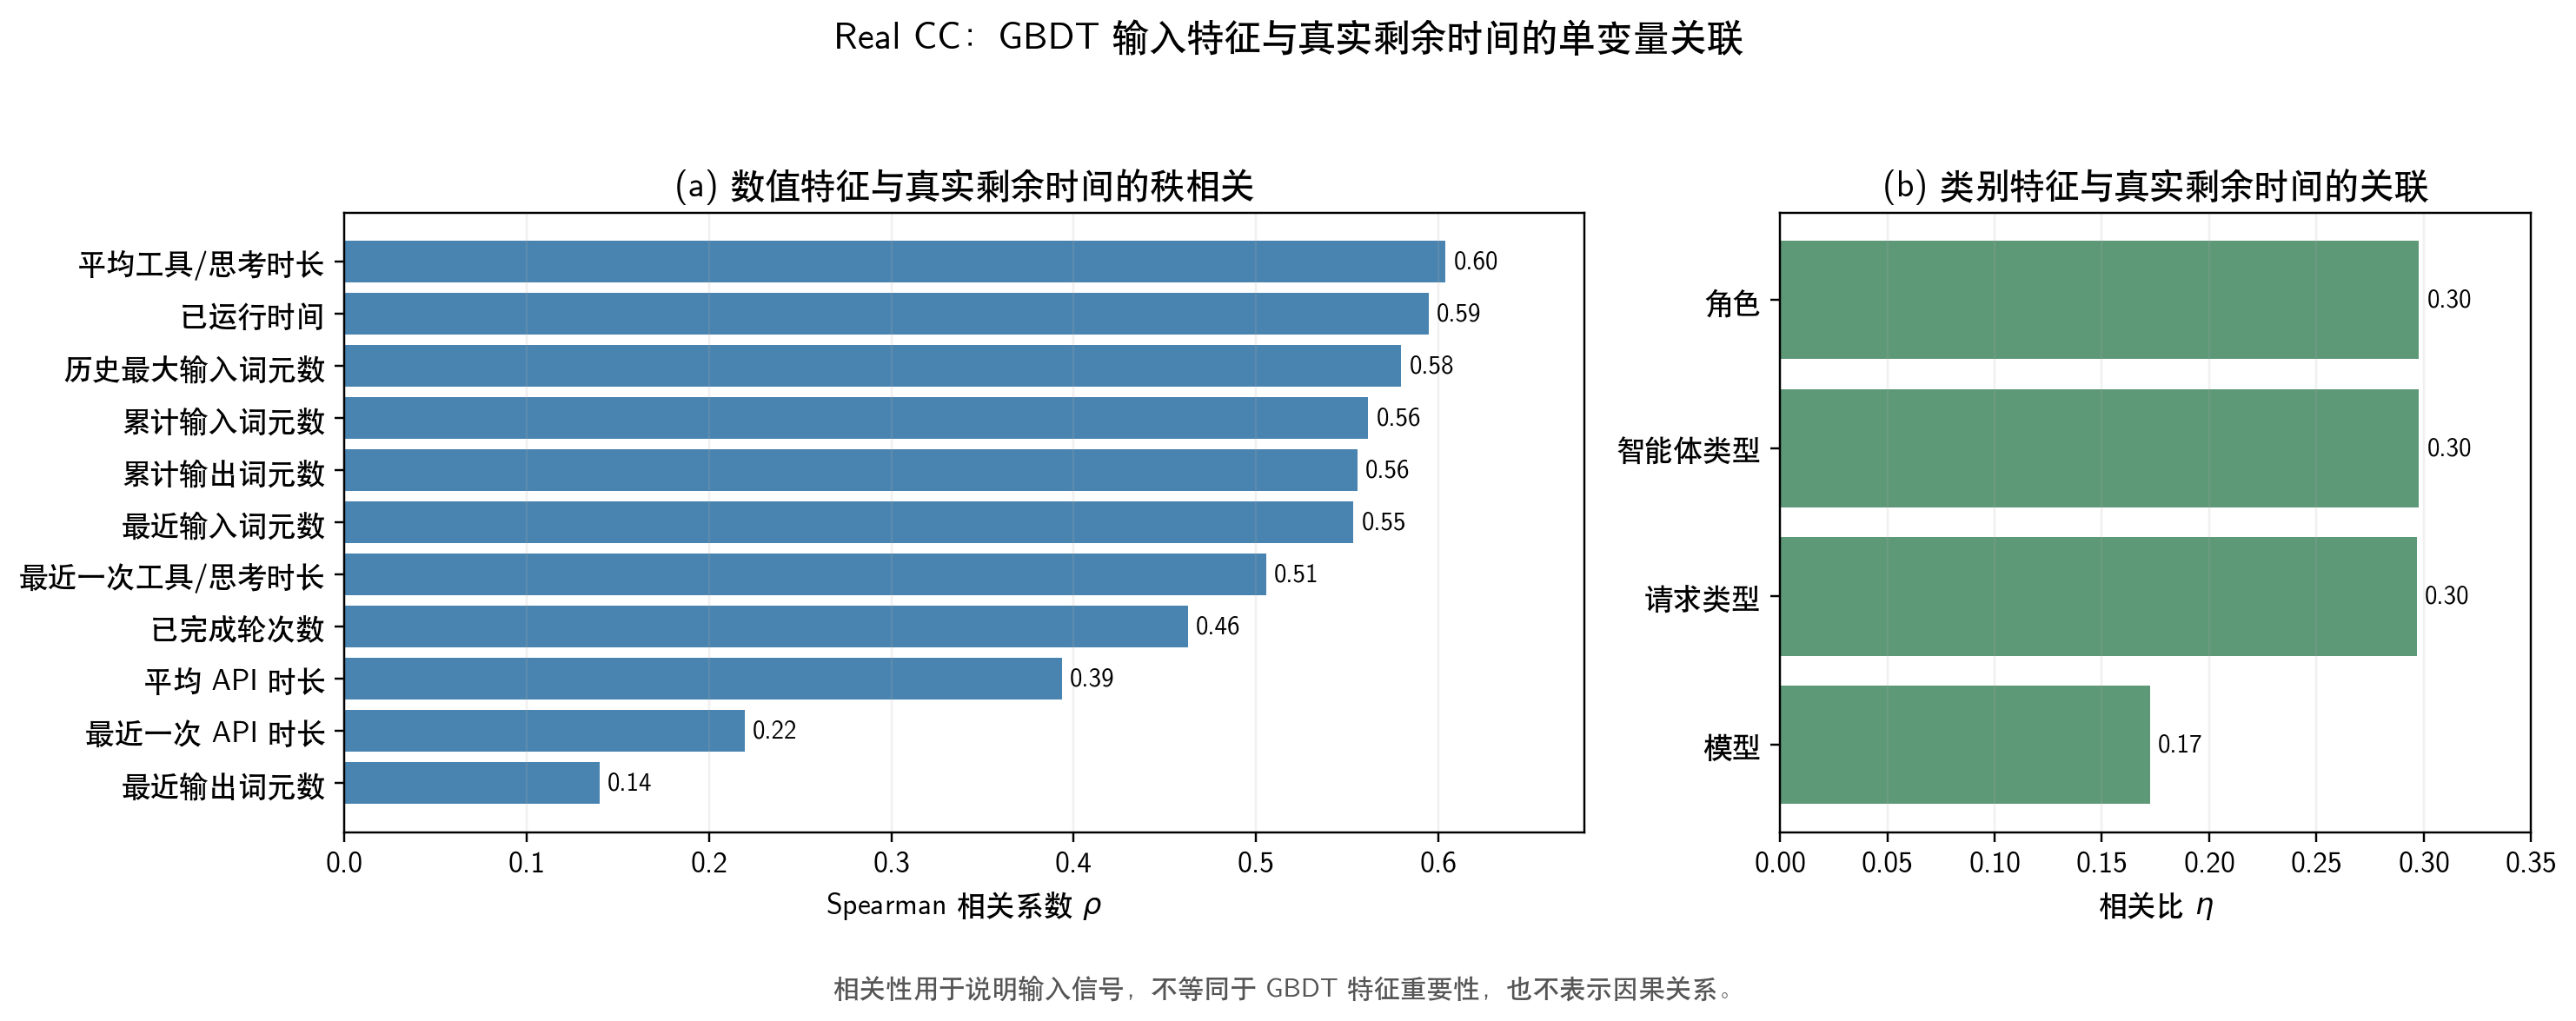
\includegraphics[width=0.99\linewidth,height=0.50\textheight,keepaspectratio]{fig_alg1_gbdt_feature_correlation.png}

  \vspace{0.02cm}
  \scriptsize
  图中数值特征使用 Spearman $\rho$，类别特征使用相关比 $\eta$；
  统计来自 393 个 Real CC 工作流的 96,103 个轮次结束样本。
  \takeaway{工具/思考时长、已运行时间和词元历史提供了最强的单变量信号；
  相关性只说明输入信号，不等同于 GBDT 特征重要性或因果关系。}
\end{frame}

\begin{frame}{算法 1 | GBDT 每轮更新后的预测准确度}
  \scriptsize
  GBDT 的模型参数在在线执行期间保持不变；每一轮结束后，系统更新
  $\phi_v(t)$ 并重新输出 P10/P50/P90，因而同一智能体的剩余时间预测
  会随新观测不断调整。下图以 P50 作为点预测。

  \vspace{0.02cm}
  \centering
  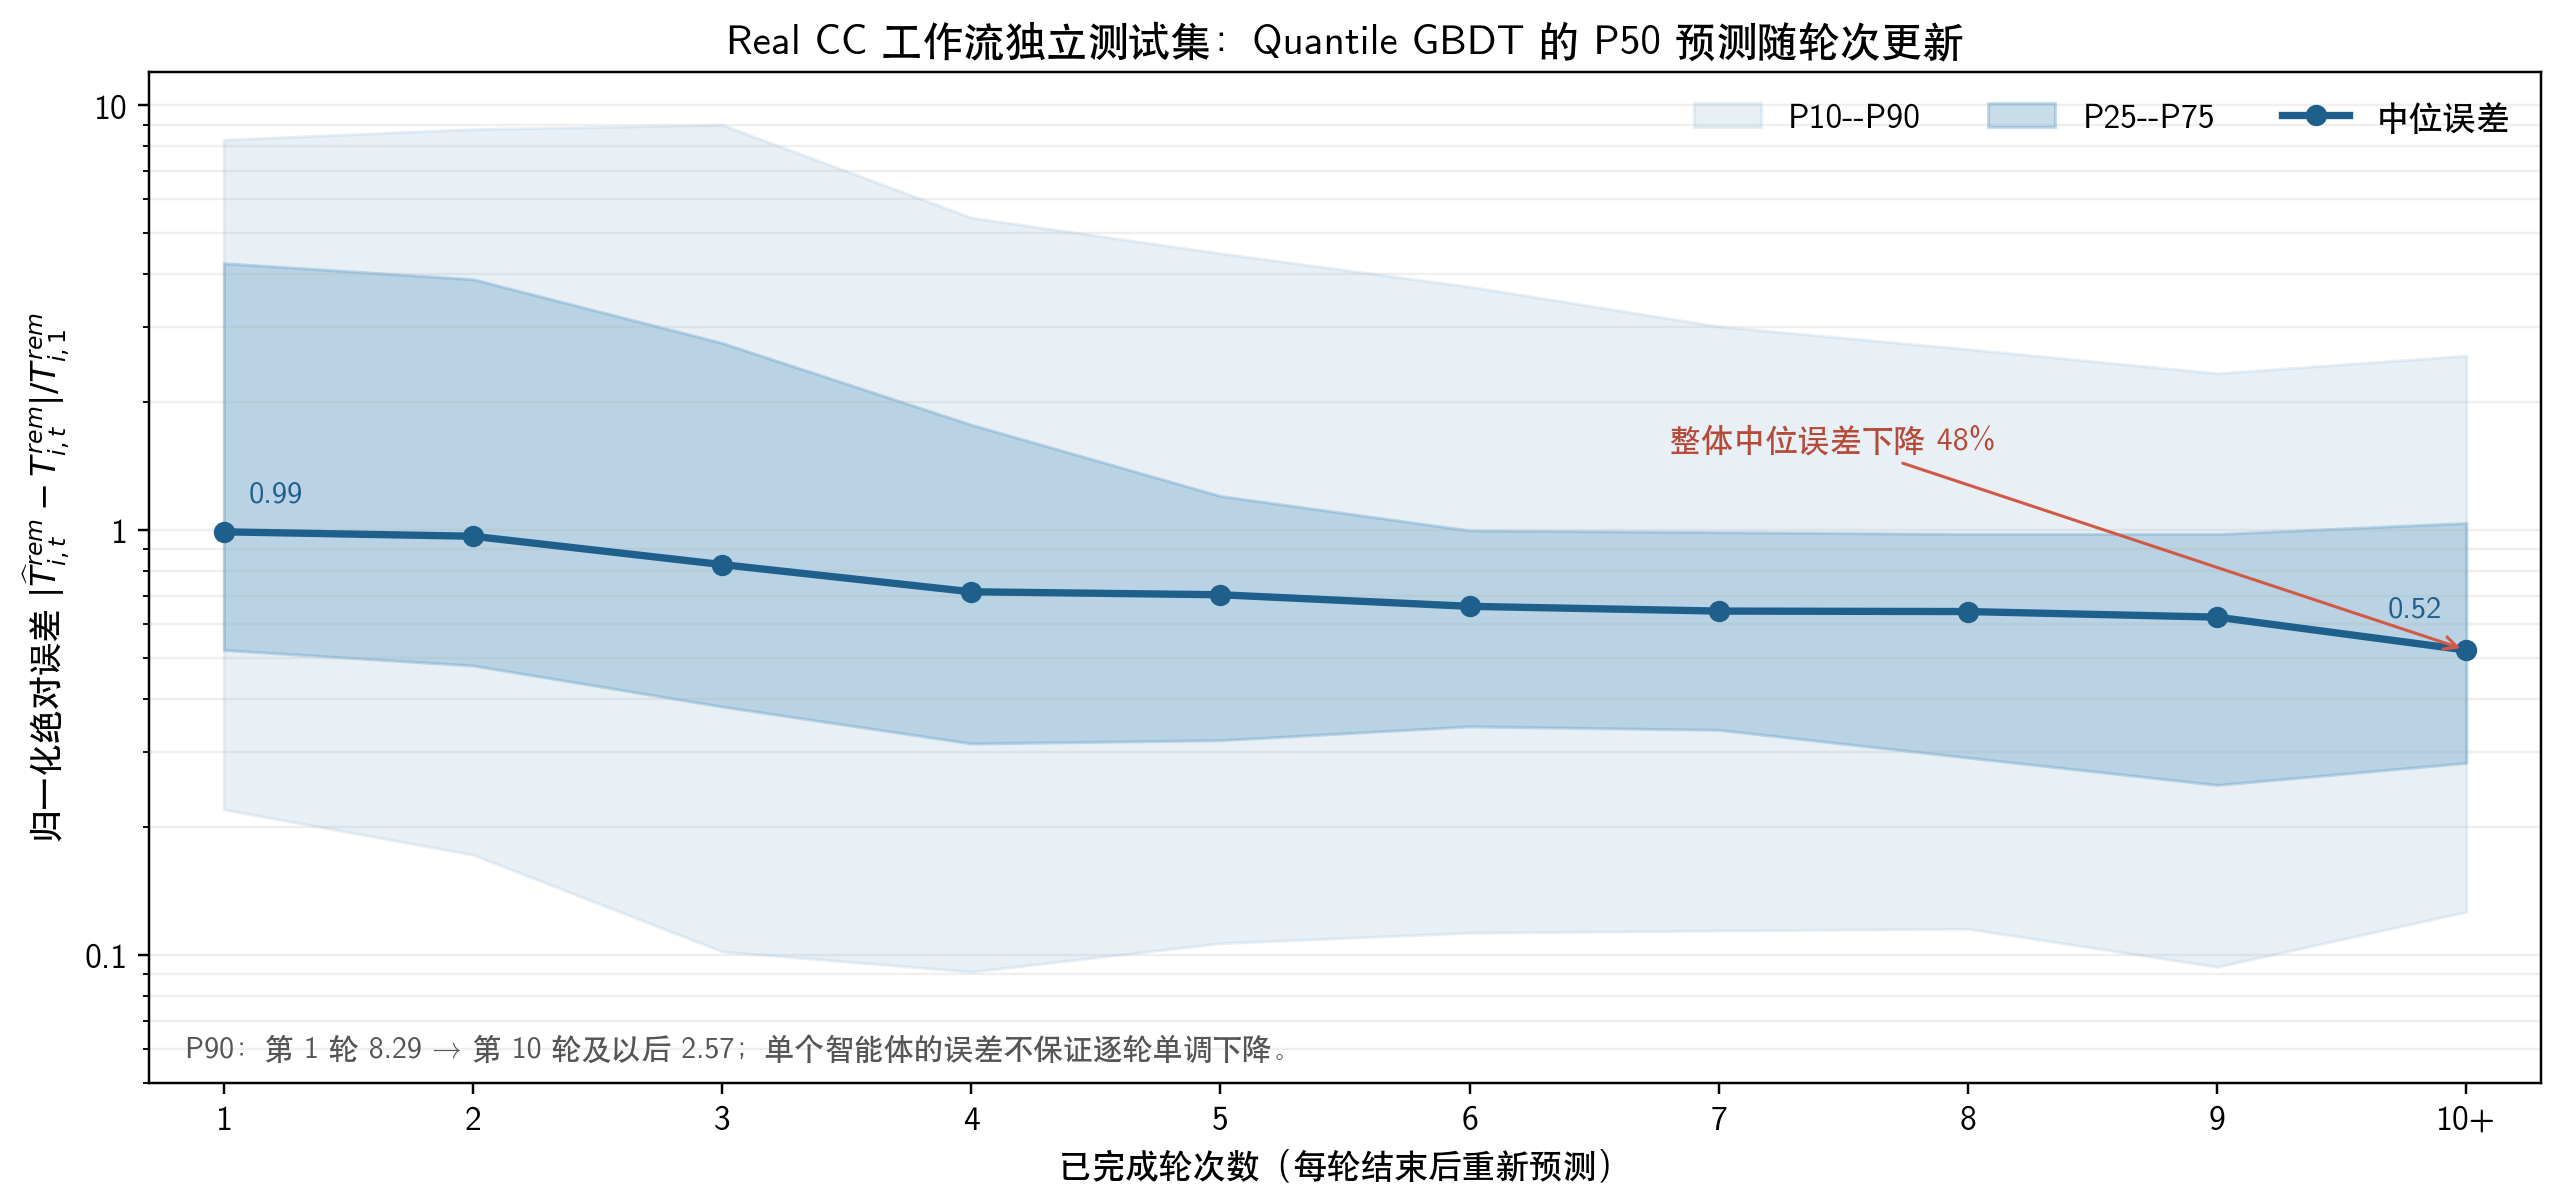
\includegraphics[width=0.99\linewidth,height=0.52\textheight,keepaspectratio]{fig_alg1_gbdt_accuracy_progress.png}

  \vspace{0.01cm}
  \scriptsize
  误差定义为
  $e_{i,t}=\lvert\widehat T_{i,t}^{\mathrm{rem}}-T_{i,t}^{\mathrm{rem}}\rvert/
  T_{i,1}^{\mathrm{rem}}$，使用每个智能体第一次预测时的真实剩余时间归一化。
  测试集包含 82 个与训练集工作流不重叠的工作流、17,074 个预测样本。
  \takeaway{总体中位误差由第 1 轮的 0.99 降至第 10 轮及以后的 0.52，
  P90 由 8.29 降至 2.57；总体准确度随信息积累改善，但单个智能体
  不保证逐轮单调改善。}
\end{frame}

\begin{frame}{算法 1 | CPM 入门：ES、EF、LS、LF 与 $S_v$}
  \small
  \textbf{CPM (Critical Path Method, 关键路径法)}：给定一个 DAG 和每个节点
  的执行时长，找出决定工作流完成时间的最长依赖路径，并计算每个
  节点在不拖慢工作流的前提下还能延迟多久。

  \vspace{0.08cm}
  \begin{columns}[T,onlytextwidth]
    \begin{column}{0.57\textwidth}
      \scriptsize
      \renewcommand{\arraystretch}{1.14}
      \begin{tabularx}{\linewidth}{p{0.13\linewidth}p{0.25\linewidth}X}
        \toprule
        符号 & 术语全称 & 直观含义 \\
        \midrule
        $ES_v$ & Earliest Start & 所有前驱完成后，$v$ 最早何时开始 \\
        $EF_v$ & Earliest Finish & 最早何时完成；$EF_v=ES_v+d_v$ \\
        $LS_v$ & Latest Start & 不增加 WCT 时，$v$ 最晚何时开始 \\
        $LF_v$ & Latest Finish & 不增加 WCT 时，$v$ 最晚何时完成 \\
        $S_v$ & Total Slack & 可吸收的额外延迟；
          $S_v=LS_v-ES_v=LF_v-EF_v$ \\
        \bottomrule
      \end{tabularx}
    \end{column}
    \begin{column}{0.40\textwidth}
      \centering
      \scriptsize
      \textbf{同一个节点的两种合法排程}

      \vspace{0.10cm}
      \begin{tikzpicture}[x=0.72cm,y=0.72cm,font=\tiny]
        \draw[-{Stealth[length=1.6mm]},draw=AegisGray] (0,0) -- (6.1,0)
          node[right] {$t$};
        \draw[fill=AegisBlueLight,draw=AegisBlue,thick]
          (0.7,1.05) rectangle (3.0,1.65);
        \node at (1.85,1.35) {时长 $d_v$};
        \node[below] at (0.7,1.05) {$ES_v$};
        \node[below] at (3.0,1.05) {$EF_v$};
        \node[left] at (0.4,1.35) {最早};

        \draw[fill=AegisOrangeLight,draw=AegisOrange,thick]
          (3.2,-0.05) rectangle (5.5,0.55);
        \node at (4.35,0.25) {时长 $d_v$};
        \node[below] at (3.2,-0.05) {$LS_v$};
        \node[below] at (5.5,-0.05) {$LF_v$};
        \node[left] at (2.9,0.25) {最晚};

        \draw[<->,draw=AegisGreen,thick]
          (0.7,2.0) -- (3.2,2.0)
          node[midway,above] {$S_v=LS_v-ES_v$};
        \draw[dashed,draw=AegisGreen] (0.7,1.7) -- (0.7,2.1);
        \draw[dashed,draw=AegisGreen] (3.2,0.65) -- (3.2,2.1);
      \end{tikzpicture}

      \vspace{0.08cm}
      \begin{beamercolorbox}[rounded=true,sep=0.75ex,wd=\linewidth]{block body}
        \scriptsize
        \textbf{前向计算：}计算 $ES/EF$ 与 WCT $L$。\par
        \textbf{后向计算：}从 $L$ 倒推 $LF/LS$。\par
        \textbf{关键节点：}$S_v=0$，不能再延迟。
      \end{beamercolorbox}
    \end{column}
  \end{columns}

  \vspace{0.06cm}
  \takeaway{松弛时间是节点的时间余量，不是执行时长；关键路径上的节点没有余量。}
\end{frame}

\begin{frame}{算法 1 | 前向计算：逐节点计算 $ES/EF$ 与 WCT}
  \small
  对式~\eqref{eq:fixed-residual-dag} 的一组时长实现值
  $\boldsymbol d^{(k)}=\{d_v^{(k)}\}$，按拓扑序从源节点向汇节点扫描：
  \begin{equation}
    ES_v^{(k)}
    =
    \max_{u\in\operatorname{pred}(v)}EF_u^{(k)},
    \qquad
    EF_v^{(k)}=ES_v^{(k)}+d_v^{(k)},
    \qquad
    L^{(k)}=\max_{z\in\operatorname{sink}}EF_z^{(k)}.
    \label{eq:cpm-forward}
  \end{equation}

  \scriptsize
  \centering
  \renewcommand{\arraystretch}{1.10}
  \begin{tabular}{lccccc}
    \toprule
    节点 $v$ & $d_v$ & 前驱节点 & $ES_v$ 的计算 & $ES_v$ & $EF_v$ \\
    \midrule
    Main & 3s  & --     & 源节点取 0         & 0  & 3  \\
    A    & 9s  & Main   & $EF_{\mathrm{Main}}$ & 3  & 12 \\
    B    & 6s  & Main   & $EF_{\mathrm{Main}}$ & 3  & 9  \\
    C    & 12s & Main   & $EF_{\mathrm{Main}}$ & 3  & 15 \\
    D    & 5s  & A, B   & $\max(12,9)$         & 12 & 17 \\
    E    & 6s  & B, C   & $\max(9,15)$         & 15 & 21 \\
    F    & 3s  & D, E   & $\max(17,21)$        & 21 & 24 \\
    \bottomrule
  \end{tabular}

  \vspace{0.10cm}
  \begin{columns}[T,onlytextwidth]
    \begin{column}{0.48\textwidth}
      \textbf{$ES_v$ 为什么取最大值？}\\
      $v$ 必须等待所有前驱节点完成，最晚完成的前驱决定其最早开始时间。
    \end{column}
    \begin{column}{0.48\textwidth}
      \textbf{工作流完成时间：}\\
      汇节点 F 的 $EF_F=24$s，因此本组实现值的剩余 WCT 为 $L=24$s。
    \end{column}
  \end{columns}
\end{frame}

\begin{frame}{算法 1 | 后向计算：计算 $LS/LF/S_v$ 与关键路径}
  \small
  令每个汇节点的 $LF=L$，再按逆拓扑序从汇节点向源节点扫描：
  \begin{equation}
    LF_v^{(k)}
    =
    \min_{z\in\operatorname{succ}(v)}LS_z^{(k)},
    \qquad
    LS_v^{(k)}=LF_v^{(k)}-d_v^{(k)},
    \qquad
    S_v^{(k)}
    =
    LS_v^{(k)}-ES_v^{(k)}
    =
    LF_v^{(k)}-EF_v^{(k)}.
    \label{eq:cpm-backward}
  \end{equation}

  \scriptsize
  \centering
  \renewcommand{\arraystretch}{1.08}
  \begin{tabularx}{0.94\textwidth}{lrrrrrX}
    \toprule
    节点 & $ES$ & $EF$ & $LS$ & $LF$ & $S_v$ & 解释 \\
    \midrule
    \textcolor{AegisRed}{\textbf{Main}} & 0  & 3  & 0  & 3  & \textbf{0} & 关键节点 \\
    A                                  & 3  & 12 & 7  & 16 & 4          & 可延迟至多 4s \\
    B                                  & 3  & 9  & 9  & 15 & 6          & 可延迟至多 6s \\
    \textcolor{AegisRed}{\textbf{C}}   & 3  & 15 & 3  & 15 & \textbf{0} & 关键节点 \\
    D                                  & 12 & 17 & 16 & 21 & 4          & 可延迟至多 4s \\
    \textcolor{AegisRed}{\textbf{E}}   & 15 & 21 & 15 & 21 & \textbf{0} & 关键节点 \\
    \textcolor{AegisRed}{\textbf{F}}   & 21 & 24 & 21 & 24 & \textbf{0} & 关键节点 \\
    \bottomrule
  \end{tabularx}

  \vspace{0.08cm}
  \begin{columns}[T,onlytextwidth]
    \begin{column}{0.48\textwidth}
      \textbf{$LF_v$ 为什么取最小值？}\\
      $v$ 必须赶在所有后继节点的 $LS$ 之前完成，最早的截止时间约束它。
    \end{column}
    \begin{column}{0.48\textwidth}
      \textbf{读表方法：}\\
      A 若额外延迟 4s，WCT 仍为 24s；C 若额外延迟 1s，WCT 就变为 25s。
    \end{column}
  \end{columns}

  \vspace{0.06cm}
  \takeaway{$S_v=0$ 的 Main $\rightarrow$ C $\rightarrow$ E $\rightarrow$ F 构成关键路径；
  一次 CPM 的复杂度为 $O(|V|+|E|)$。}
\end{frame}

\begin{frame}{算法 1 | 固定 DAG 松弛时间：只采样智能体剩余时间}
  \small
  固定式~\eqref{eq:fixed-residual-dag} 的拓扑，只从校准分布生成
  $K$ 组时长实现值，并分别运行 CPM：
  \begin{equation}
    d_v^{(k)}\sim F_v(t),
    \qquad
    \sigma_r^{(k)}(t)
    =
    S_{v(r)}\!\left(D_w^{\mathrm{rem}}(t),\boldsymbol d^{(k)}\right),
    \qquad
    \widehat\sigma_r(t)
    =
    Q_{q_\sigma}
    \!\left(
      \{\sigma_r^{(k)}(t)\}_{k=1}^{K}
    \right).
    \label{eq:request-slack}
  \end{equation}

  \begin{columns}[T,onlytextwidth]
    \begin{column}{0.47\textwidth}
      \scriptsize
      \textbf{固定拓扑}
      \begin{itemize}\tightitems
        \item 完整 $D_w$ 在工作流启动时已知；
        \item 所有边固定（等价 $p_e=1$），拓扑序可复用；
        \item 每组样本不改变节点或边；
        \item 节点完成只改变剩余节点集合。
      \end{itemize}
    \end{column}
    \begin{column}{0.50\textwidth}
      \scriptsize
      \textbf{唯一预测目标：智能体执行片段的剩余时间}
      \begin{itemize}\tightitems
        \item 用角色/类型、轮次数、已运行时间、词元数、
          工具/API 延迟与负载构造 $\phi_v(t)$；
        \item 预测器发布校准后的 $F_v(t)$，而不是单一点估计；
        \item 对每组 $\boldsymbol d^{(k)}$ 运行 CPM；
        \item $Q_{q_\sigma}$ 取低分位数，得到保守的请求松弛时间。
      \end{itemize}
    \end{column}
  \end{columns}

  \vspace{0.07cm}
  \boundary{拓扑不确定性不属于当前问题；动态分支或额外反馈轮次
  必须先编译成另一个固定 DAG，不能在一次工作流执行中改变图结构。}
\end{frame}

\begin{frame}{算法 1 | 在线过程与版本化输出}
  \begin{paperalgo}{算法 1：固定 DAG 工作流松弛时间估计}
    \algline{工作流启动前，用任务分解适配器或角色协议适配器构造固定 $D_w$，并发布不可变的 \code{dag\_version}。}
    \algline{根据轮次/节点进度更新待执行、执行中、已完成状态与式~\eqref{eq:fixed-residual-dag}。}
    \algline{按式~\eqref{eq:node-duration} 构造特征，并由 Quantile GBDT 更新 $F_v(t)$。}
    \algline{采样 $K$ 组智能体时长；每组用式~\eqref{eq:cpm-forward}--\eqref{eq:cpm-backward} 计算节点松弛时间。}
    \algline{按式~\eqref{eq:request-slack} 发布执行中请求的松弛时间分位数。}
    \algline{每次进度或时长模型更新只递增 \code{slack\_version}；\code{dag\_version} 保持不变。}
  \end{paperalgo}

  \vspace{0.06cm}
  \scriptsize
  \renewcommand{\arraystretch}{1.12}
  \begin{tabularx}{\textwidth}{p{0.20\textwidth}X}
    \toprule
    执行片段字段 & \code{workflow\_id}, \code{dag\_node\_id},
    \code{agent\_instance\_id}, \code{role}, \code{subtask\_id},
    \code{activation\_id}, \code{edge\_type}, \code{dag\_version} \\
    输出字段 &
    \code{predicted\_slack\_ms}, \code{slack\_quantile},
    \code{slack\_version} \\
    诊断字段 & \code{remaining\_p10/p50/p90}, \code{interval\_coverage},
    \code{prediction\_timestamp} \\
    过期策略 & 路由只接受单调不减的版本；超时快照按零松弛时间处理 \\
    \bottomrule
  \end{tabularx}
\end{frame}

% !TeX root = ../paper_outline.tex
\section{算法 2：DP rank 内的松弛感知 KV 块备份决策}

\begin{frame}{算法 2 | 符号、动作与窗口预算}
  \scriptsize
  Router 先用 Cache-Aware 排名为请求 $r$ 固定执行 Rank 与 Backup Rank：
  \begin{equation}
    \boldsymbol\pi_r(t)=\operatorname{Rank}_{\mathrm{CA}}
      \!\left(r;\{L_d(t),\mathcal T_d(t)\}_{d\in\mathcal A(t)}\right),
    \quad e(r)=\pi_{r,1},\quad b(r)=\pi_{r,2}.
    \label{eq:router-top2}
  \end{equation}
  算法 2 不再选择目的 Rank；它在 DP rank 内为已提交 KV 块选择 L1、L2 或重计算。
  KV 块表示为：
  \begin{equation}
    s=
    \bigl(
      o_s,[i_s,j_s),v_s,b_s,\mathcal R_s(t)
    \bigr),
    \qquad 0<b_s\le b_0.
    \label{eq:segment-tuple}
  \end{equation}

  \tiny
  \renewcommand{\arraystretch}{1.00}
  \begin{tabularx}{\textwidth}{p{0.22\textwidth}X}
    \toprule
    符号 & 含义 \\
    \midrule
    $o_s,[i_s,j_s),v_s$ & 所有者故障域、词元区间与版本 \\
    $b_s,b_0$ & 当前块字节数与固定块大小上限 \\
    $\mathcal R_s(t)$ & 时刻 $t$ 引用块 $s$ 的活跃请求集合 \\
    $L_d(t),\mathcal T_d(t),\mathcal A(t)$ & Rank $d$ 的正常推理负载、Router 侧 Radix Tree 与健康 Rank 集合 \\
    $e(r),b(r)$ & Router 给请求 $r$ 固定的执行 Rank 与 Backup Rank \\
    $n=b(r_s)$ & 引用块 $s$ 的请求所绑定的唯一 Backup DP rank \\
    $a\in\{B_1,B_2,R\}$ & L1 Backup、L2 Backup 或 Recompute \\
    $x_{s,n,a}^{(k)}$ & 算法 2 是否计划在已给定 Rank $n$ 上采用动作 $a$ \\
    $z_{s,n,a}^{(k)}$ & 目标 Rank 完成复制并 ACK 后的提交状态，且 $z\le x$ \\
    $\alpha_n^{(k)},\beta_n^{(k)}$ & 算法 3 为当前窗口发布的 L1/L2 备份比例 \\
    $D_{n,1}^{(k)},D_{n,2}^{(k)}$ & 算法 2 发布的容量截断前逐层影子需求 \\
    \bottomrule
  \end{tabularx}

  \vspace{0.02cm}
  \boundary{Router 只绑定请求级 Backup Rank；算法 2 只在该 Rank 内选择 KV 块的 L1/L2/Recompute 动作。}
\end{frame}

\begin{frame}{算法 2 | 目标覆盖与恢复时延}
  \small
  Router 已给定的 Backup Rank $n=b(r_s)$ 可能拥有该块的有效前缀；实际需要复制的字节数为：
  \begin{equation}
    m_{s,n,a}
    =
    \left[
      b_s-\operatorname{covered\_bytes}(s,n,a)
    \right]_+.
    \label{eq:missing-bytes}
  \end{equation}
  对动作 $a\in\{B_1,B_2,R\}$，故障时的重试时延定义为：
  \begin{equation}
    R_{s,n,a}
    =
    \begin{cases}
      q_{n,B_1}^{\mathrm{rec}}+
      m_{s,n,B_1}/BW_{n,B_1}^{\mathrm{P2P}}+R_s^{\mathrm{tail}},
      & a=B_1,\\
      q_{n,B_2}^{\mathrm{rec}}+
      m_{s,n,B_2}/BW_{n,B_2}^{\mathrm{H2D}}+R_s^{\mathrm{tail}},
      & a=B_2,\\
      R_s^{\mathrm{prefill}}+R_s^{\mathrm{tail}},
      & a=R.
    \end{cases}
    \label{eq:recovery-latency}
  \end{equation}

  \scriptsize
  式~\eqref{eq:missing-bytes} 中 $[\cdot]_+=\max(\cdot,0)$；
  $q^{\mathrm{rec}}$ 是恢复建立与排队时间，$BW$ 是实测有效带宽，
  $R_s^{\mathrm{prefill}}$ 是从输入重建该块的时间，
  $R_s^{\mathrm{tail}}$ 是安全恢复前沿之后不可避免的重放时间。
  KV 流式复制与加载-重算权衡的系统依据分别见
  DejaVu 与 Cake\cite{strati2024dejavu,jin2025cake}。
\end{frame}

\begin{frame}{算法 2 | 松弛感知的工作流惩罚}
  \small
  算法 1 发布的 $\widehat\sigma_r(t)$ 表示请求 $r$ 可被延迟而不增加
  工作流完成时间的预算。动作 $a$ 的可见惩罚为：
  \begin{equation}
    P_{s,n,a}(t)
    =
    \sum_{w\in\mathcal W_s}
    \max_{r\in\mathcal R_s(t)\cap\mathcal R_w}
    \left[
      R_{s,n,a}-\widehat\sigma_r(t)
    \right]_+.
    \label{eq:slack-penalty}
  \end{equation}

  \scriptsize
  $\mathcal W_s$ 是引用块 $s$ 的工作流集合；同一工作流内取最大值，
  避免共享块被重复计入同一个工作流完成时间；不同工作流之间再求和。
  单请求时，式~\eqref{eq:slack-penalty} 退化为
  $P_{s,n,a}=[R_{s,n,a}-\widehat\sigma_r]_+$。

  \vspace{0.10cm}
  \renewcommand{\arraystretch}{1.16}
  \begin{tabularx}{\textwidth}{p{0.27\textwidth}X}
    \toprule
    松弛区间 & 备份决策含义 \\
    \midrule
    $\widehat\sigma_r\ge R_{s,R}$ & 重计算延迟可被隐藏，块通常保持 Recompute \\
    $R_{s,B_2}\le\widehat\sigma_r<R_{s,R}$ & L1/L2 都产生正恢复收益 \\
    $R_{s,B_1}\le\widehat\sigma_r<R_{s,B_2}$ & L1 的可见恢复收益明显高于 L2 \\
    $\widehat\sigma_r<R_{s,B_1}$ & 三条路径都可见，按净恢复收益选择动作 \\
    \bottomrule
  \end{tabularx}
\end{frame}

\begin{frame}{算法 2 | 恢复路径性能}
  \centering
  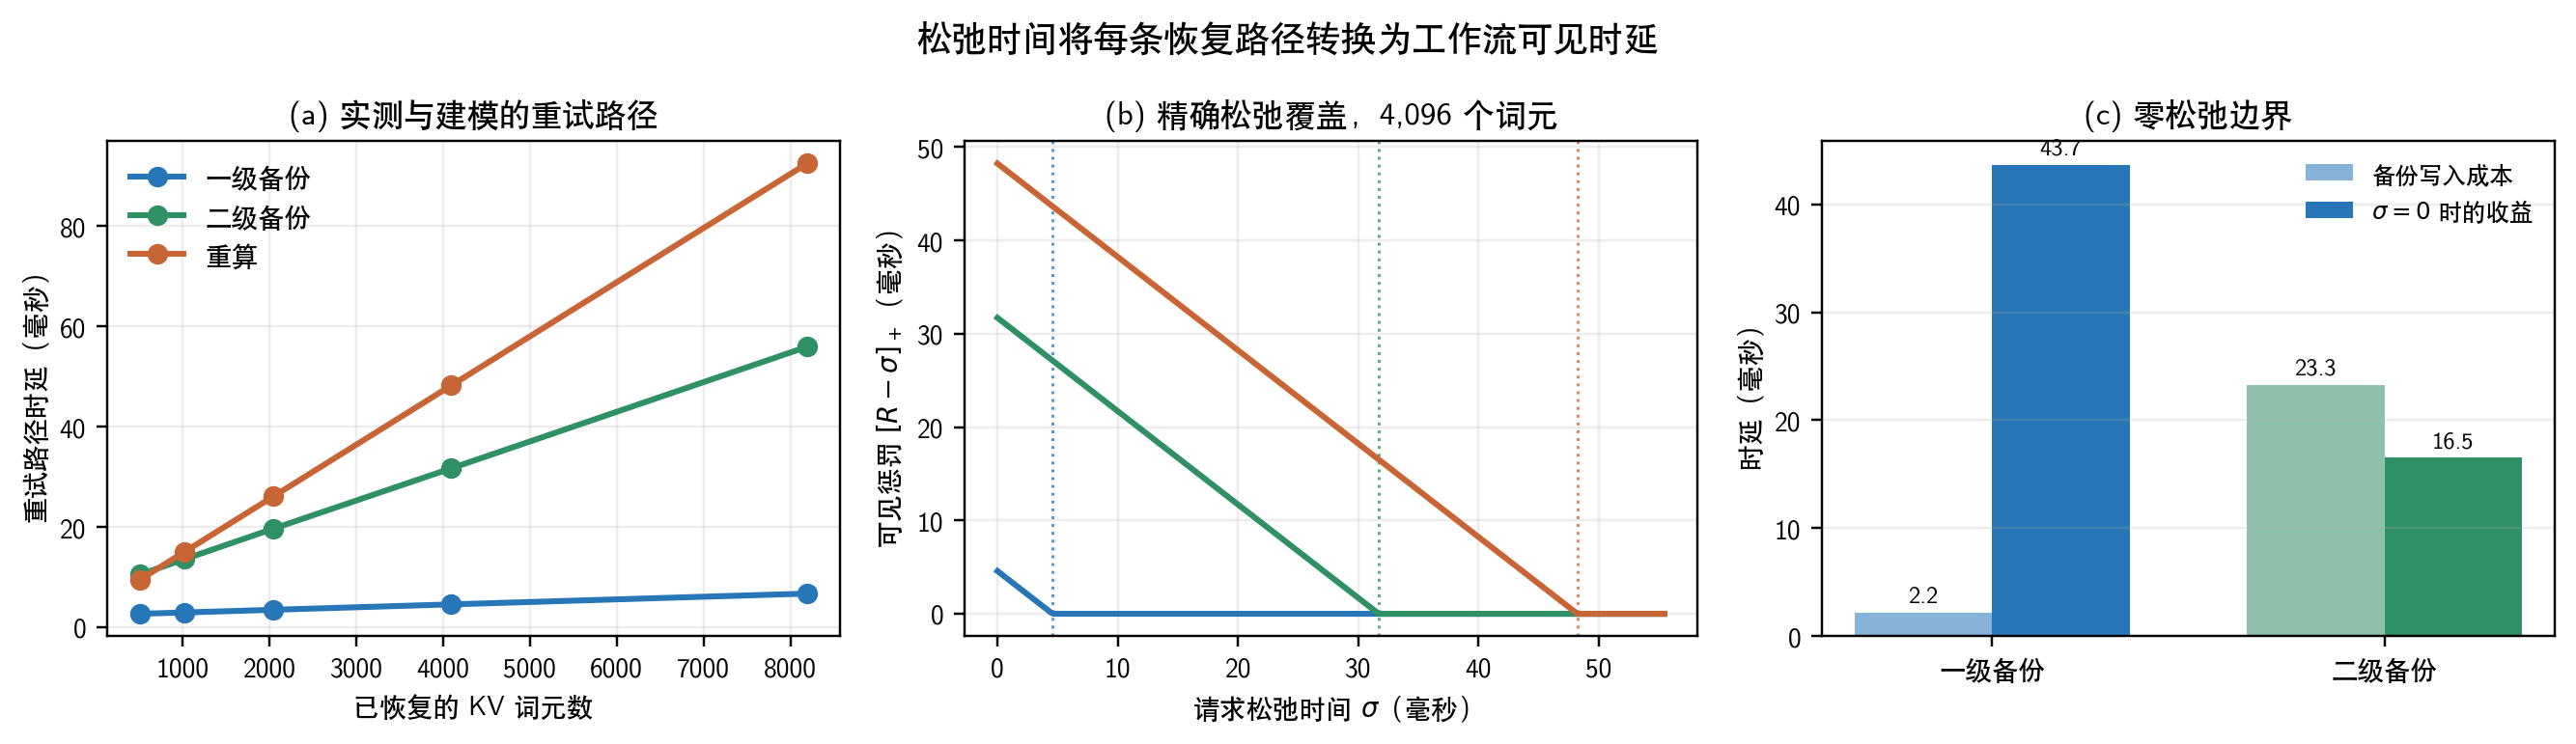
\includegraphics[width=0.98\linewidth,height=0.73\textheight,keepaspectratio]{fig_alg2_slack_coverage.png}

  \vspace{0.02cm}
  \scriptsize
  两级备份路径使用 3 次 SGLang CUDA 数据搬运微基准的 p50 聚合值与固定建立时延；
  重算使用 SGLSim 系数模型。对于 4,096 词元的 KV 块，
  $R_{B_1}=4.58$ms、$R_{B_2}=31.71$ms、$R_R=48.24$ms。

  \vspace{0.04cm}
  \takeaway{松弛时间跨过 $R_{B_1}$、$R_{B_2}$、$R_R$ 时，
  同一 KV 块在各恢复层的收益和最终动作随之变化。}
\end{frame}

\begin{frame}{算法 2 | 恢复收益与候选项密度}
  \small
  相对重算，备份动作 $a\in\{B_1,B_2\}$ 的恢复收益、写入成本与净收益为：
  \begin{equation}
    \begin{aligned}
      G_{s,n,a}(t)
        &=\left[P_{s,R}(t)-P_{s,n,a}(t)\right]_+,\\
      C_{s,n,a}^{\mathrm{write}}
        &=q_{n,a}^{\mathrm{write}}
          +\frac{m_{s,n,a}}{BW_{o_s,n,a}^{\mathrm{write}}},\\
      V_{s,n,a}(t)
        &=p_sG_{s,n,a}(t)-\lambda_a C_{s,n,a}^{\mathrm{write}}.
    \end{aligned}
    \label{eq:recovery-benefit}
  \end{equation}
  在线实现按单位增量字节的净收益排序：
  \begin{equation}
    \rho_{s,n,a}(t)
      =
      \frac{V_{s,n,a}(t)}
           {\max(m_{s,n,a},1)}.
    \label{eq:chunk-priority}
  \end{equation}

  \scriptsize
  $p_s$ 是所有者在块生命周期内的故障概率；
  $\lambda_a$ 把正常路径写入开销换算为目标代价。
  只有 $V_{s,n,a}>0$ 的候选项进入备份决策；$\rho$ 用于在线 admit/replace，
  但算法 2 的输出是容量约束后的动作，而不只是排序结果。
\end{frame}

\begin{frame}{算法 2 | 核心公式拆解：收益、成本与单位容量价值}
  \begin{columns}[T,onlytextwidth]
    \begin{column}{0.59\textwidth}
      \begin{beamercolorbox}[rounded=true,sep=1.0ex,wd=\linewidth]{block body}
        \small
        \begin{align*}
          G_{s,n,a}(t)
            &=\left[P_{s,R}(t)-P_{s,n,a}(t)\right]_+,\\[0.35em]
          C_{s,n,a}^{\mathrm{write}}
            &=q_{n,a}^{\mathrm{write}}
              +\frac{m_{s,n,a}}{BW_{o_s,n,a}^{\mathrm{write}}},\\[0.35em]
          V_{s,n,a}(t)
            &=p_sG_{s,n,a}(t)-\lambda_a C_{s,n,a}^{\mathrm{write}},\\[0.35em]
          \rho_{s,n,a}(t)
            &=\frac{V_{s,n,a}(t)}{\max(m_{s,n,a},1)}.
        \end{align*}
      \end{beamercolorbox}

      \vspace{0.14cm}
      \scriptsize
      这里 $n=b(r_s)$ 已由 Router 固定；算法 2 比较的是同一 Backup Rank 内
      的 $B_1/B_2/R$，不是在不同 Rank 之间重新选目的地。
    \end{column}
    \begin{column}{0.38\textwidth}
      \layercard{AegisBlue}{1. $G$：恢复收益}{相对 Recompute，动作 $a$ 能减少多少可见工作流惩罚。}
      \vspace{0.08cm}
      \layercard{AegisOrange}{2. $C$：备份成本}{目标端排队/建立时间，加上未覆盖字节的实际复制时间。}
      \vspace{0.08cm}
      \layercard{AegisGreen}{3. $V$：净收益}{故障概率加权的恢复收益，减去正常路径写入代价。}
      \vspace{0.08cm}
      \layercard{AegisPurple}{4. $\rho$：单位容量价值}{每增加一个 Backup 字节可获得的净收益，用于 admit/replace。}
    \end{column}
  \end{columns}

  \vspace{0.12cm}
  \boundary{$V\le0$ 的动作不备份；$V>0$ 时再由 $\rho$ 和当前 $\alpha_n/\beta_n$ 配额决定是否提交。}
\end{frame}

\begin{frame}{算法 2 | 当前窗口的容量约束备份决策}
  \small
  对每个目标 DP rank $n$，令
  $\mathcal S_n^{(k)}=\{s:b(r_s)=n\}$。窗口 $k$ 只在该 Rank 内选择层级：
  \begin{equation}
    \begin{aligned}
      \max_{\mathbf x_n^{(k)}}\quad
        &\sum_{s\in\mathcal S_n^{(k)}}\sum_{a\in\{B_1,B_2\}}
          V_{s,n,a}^{(k)}x_{s,n,a}^{(k)},\\
      \text{s.t.}\quad
        &\sum_{s\in\mathcal S_n^{(k)}}m_{s,n,B_1}x_{s,n,B_1}^{(k)}
          \le\alpha_n^{(k)}M_n,\\
        &\sum_{s\in\mathcal S_n^{(k)}}m_{s,n,B_2}x_{s,n,B_2}^{(k)}
          \le\beta_n^{(k)}H_n,\\
        &\sum_{a\in\{B_1,B_2\}}x_{s,n,a}^{(k)}\le1,
          \quad\forall s\in\mathcal S_n^{(k)},\\
        &x_{s,n,a}^{(k)}\in\{0,1\}.
    \end{aligned}
    \label{eq:backup-placement}
  \end{equation}

  \scriptsize
  未被选中的块采用 Recompute。在线实现按 $\rho$ 做 admit/replace：
  新候选项只有在净收益为正且能放入当前配额，或能替换更低密度条目时才提交。
  相同块至多选择一个层；目的 Rank 已由式~\eqref{eq:router-top2} 固定，
  算法 2 不读取 Router 的全局负载，也不改变请求级 Rank 绑定。

  \vspace{0.06cm}
  \takeaway{$\alpha_n^{(k)},\beta_n^{(k)}$ 约束窗口 $k$ 的实际备份动作。}
\end{frame}

\begin{frame}{算法 2 | 容量截断前需求与跨窗口反馈}
  \small
  为区分“当前没有需求”和“当前配额不足”，算法 2 同时构造影子选择
  $y_{s,n,a}^{(k)}$：它保留版本、健康、故障域和单块唯一动作约束，
  但暂时移除式~\eqref{eq:backup-placement} 的两条全局容量约束。
  逐节点、逐层影子需求与实际占用为：
  \begin{equation}
    \begin{aligned}
      D_{n,1}^{(k)}
        &=\sum_s m_{s,n,B_1}y_{s,n,B_1}^{(k)},&
      U_{n,1}^{(k)}
        &=\sum_s m_{s,n,B_1}z_{s,n,B_1}^{(k)},\\
      D_{n,2}^{(k)}
        &=\sum_s m_{s,n,B_2}y_{s,n,B_2}^{(k)},&
      U_{n,2}^{(k)}
        &=\sum_s m_{s,n,B_2}z_{s,n,B_2}^{(k)},\\
      O_{n,\ell}^{(k)}
        &=\left[D_{n,\ell}^{(k)}-U_{n,\ell}^{(k)}\right]_+,
        &\ell&\in\{1,2\}.
    \end{aligned}
    \label{eq:shadow-demand}
  \end{equation}

  \scriptsize
  $D$ 表示正净收益动作希望获得的容量；$U$ 只统计目标 DP rank 已 ACK 的实际占用；
  $O$ 表示尚未满足的正收益需求。ACK 的权威状态保留在目标 DP rank，
  聚合后的 Recovery Hint 异步发布给 Router，供故障时零查询重路由。

  \vspace{0.08cm}
  \centering
  \begin{tikzpicture}[
    box/.style={draw,rounded corners=2pt,align=center,font=\scriptsize,
      minimum width=2.55cm,minimum height=0.68cm,inner sep=3pt},
    arr/.style={-{Stealth[length=1.7mm]},thick,draw=AegisGray}
  ]
    \node[box,draw=AegisGreen,fill=AegisGreenLight] (b) at (0,0)
      {算法 3，窗口 $k$\\$\alpha^{(k)},\beta^{(k)}$};
    \node[box,draw=AegisOrange,fill=AegisOrangeLight] (p) at (3.7,0)
      {算法 2，窗口 $k$\\备份动作 + $D^{(k)},U^{(k)},O^{(k)}$};
    \node[box,draw=AegisGreen,fill=AegisGreenLight] (n) at (7.4,0)
      {算法 3，窗口 $k+1$\\$\alpha^{(k+1)},\beta^{(k+1)}$};
    \draw[arr] (b) -- node[above,font=\tiny]{当前配额} (p);
    \draw[arr] (p) -- node[above,font=\tiny]{需求反馈} (n);
  \end{tikzpicture}
\end{frame}

\begin{frame}{算法 2 | 在线决策流程}
  \begin{paperalgo}{算法 2：松弛感知的 KV 块备份决策}
    \algline{读取 Router 随请求发布的固定 $e(r),b(r)$；算法 2 不重新选择 Backup Rank。}
    \algline{目标 DP rank 在窗口 $k$ 读取本地算法 3 已发布的 $\alpha_n^{(k)},\beta_n^{(k)}$ 和预算版本。}
    \algline{KV 块提交或扩展时，建立可行的 L1 Backup、L2 Backup 与 Recompute 恢复路径。}
    \algline{按式~\eqref{eq:slack-penalty}--\eqref{eq:chunk-priority} 计算可见惩罚、净恢复收益和候选项密度。}
    \algline{忽略全局容量约束得到影子选择，并按式~\eqref{eq:shadow-demand} 聚合 $D_{n,1}^{(k)},D_{n,2}^{(k)}$。}
    \algline{按式~\eqref{eq:backup-placement} 的当前 L1/L2 配额执行 admit/replace，生成最终备份动作。}
    \algline{目标 DP rank 完成复制后设置 $z=1$；未选中、未 ACK、复制失败或版本失效的块保持 Recompute。}
    \algline{按请求聚合 ACK frontier，异步推送 Recovery Hint；Router 只缓存摘要，不管理 Backup 容量。}
    \algline{窗口结束时在本地发布 plan 版本及 $D^{(k)},U^{(k)},O^{(k)}$，供算法 3 决定下一窗口预算。}
  \end{paperalgo}

  \vspace{0.08cm}
  \begin{block}{窗口边界}
    \footnotesize
    算法 2 的反馈不会追溯修改窗口 $k$；它只影响算法 3 发布的窗口 $k+1$
    的 $\alpha_n,\beta_n$。
  \end{block}
\end{frame}

% !TeX root = ../paper_outline.tex
\section{算法 3：DP rank 内的反馈驱动 L1/L2 容量控制}

\begin{frame}{算法 3 | 符号与跨窗口输入}
  \scriptsize
  \renewcommand{\arraystretch}{1.08}
  \begin{tabularx}{\textwidth}{p{0.22\textwidth}p{0.18\textwidth}X}
    \toprule
    符号 & 单位/范围 & 含义 \\
    \midrule
    $M_n,H_n$ & 字节 & 节点 $n$ 可管理的 L1 显存与 L2 主机内存 \\
    $L_{n,1}^{(k)},L_{n,2}^{(k)}$ & 字节 & 窗口 $k$ 的正常 L1/L2 服务负载样本 \\
    $r_{n,1},r_{n,2}$ & 字节 & 为正常负载突发保留的安全余量 \\
    $D_{n,1}^{(k)},D_{n,2}^{(k)}$ & 字节 & 本地算法 2 在窗口 $k$ 发布的容量截断前影子需求 \\
    $U_{n,\ell}^{(k)},O_{n,\ell}^{(k)}$ & 字节 & 已 ACK 实际占用与未满足需求，$\ell\in\{1,2\}$ \\
    $Z_{n,\ell}^{(k)}$ & 字节 & 本窗口需承接的容量，$Z=U+O=\max(U,D)$ \\
    $h_{n,1},h_{n,2}$ & 字节 & 为下一窗口需求突发保留的备份余量 \\
    $\alpha_n^{(k)},\beta_n^{(k)}$ & $[0,1]$ & 窗口 $k$ 的 L1/L2 备份容量比例 \\
    \bottomrule
  \end{tabularx}

  \vspace{0.08cm}
  \small
  算法 3 在每个 DP rank 内运行；它发布的比例把本地两个资源层划分为备份区与正常服务区：
  \begin{equation}
    \begin{aligned}
      M_n^{B_1}(k)&=\alpha_n^{(k)}M_n,
      &M_n^{\mathrm{serve}}(k)&=(1-\alpha_n^{(k)})M_n,\\
      H_n^{B_2}(k)&=\beta_n^{(k)}H_n,
      &H_n^{\mathrm{cache}}(k)&=(1-\beta_n^{(k)})H_n.
    \end{aligned}
    \label{eq:tier-partition}
  \end{equation}

  \scriptsize
  \boundary{算法 3 不在 Router 上运行。它在窗口边界读取本地算法 2 的 $D^{(k)},U^{(k)},O^{(k)}$；
  发布结果从窗口 $k+1$ 起生效，不追溯改变窗口 $k$ 的备份动作。}
\end{frame}

\begin{frame}{算法 3 | 节点负载偏斜与 L1 安全上限}
  \centering
  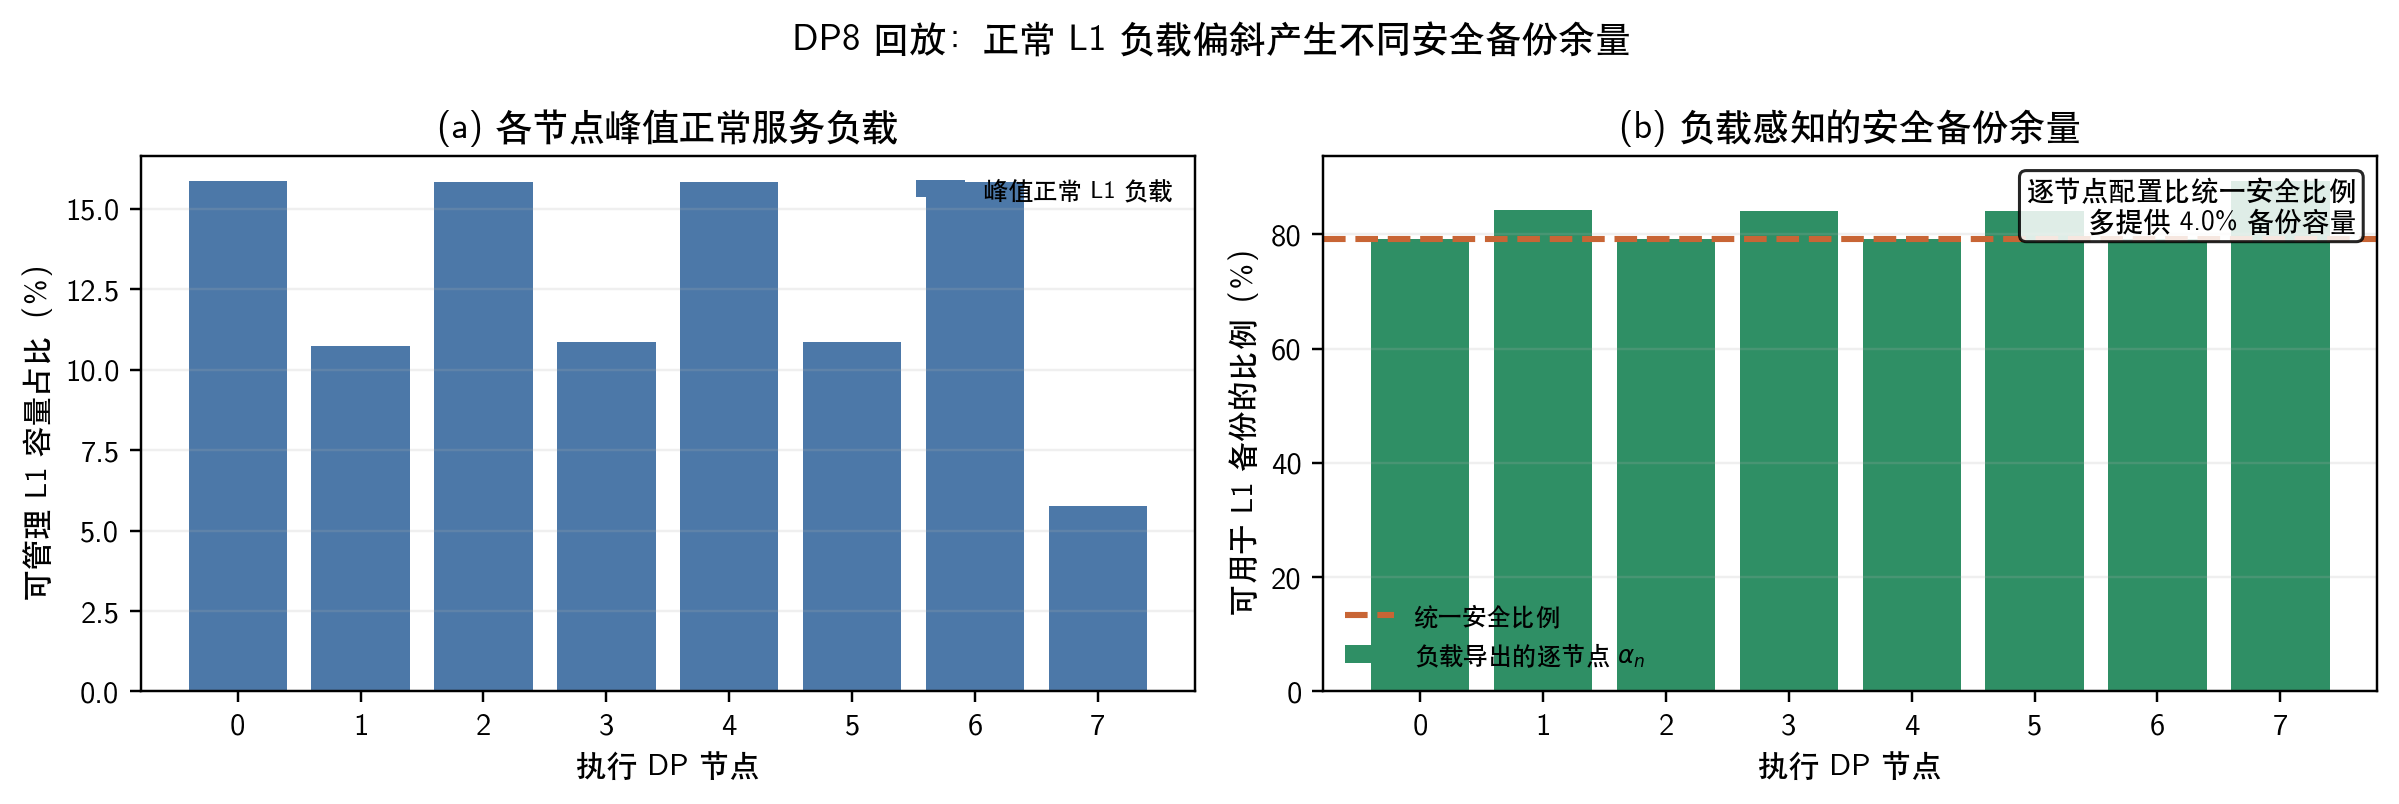
\includegraphics[width=0.98\linewidth,height=0.70\textheight,keepaspectratio]{fig_alg3_per_node_alpha.png}

  \vspace{0.02cm}
  \scriptsize
  DP8 回放根据请求存活区间与服务 KV 词元数重建各节点峰值 L1 正常负载。
  在额外保留 5\% 安全余量时，负载导出的 L1 备份比例安全上限为
  79.2\%--89.2\%；逐节点上限比统一安全上限多提供约 4.0\% 的可用容量。

  \vspace{0.03cm}
  \boundary{该图只验证算法 3 的正常负载安全上限分支，不包含算法 2 的影子需求响应。
  L2 的 $\beta_n$ 仍需要主机内存负载与联动调节实验单独验证。}
\end{frame}

\begin{frame}{算法 3 | 正常服务安全上限}
  \small
  给定正常负载风险目标 $\varepsilon_{n,1},\varepsilon_{n,2}$，先计算
  窗口 $k+1$ 可用于备份的安全上限：
  \begin{equation}
    \begin{aligned}
      A_{n}^{\mathrm{safe},(k+1)}
        &=
        \min\!\left(
          \alpha_n^{\max},
          \left[
            \frac{M_n-Q_{1-\varepsilon_{n,1}}(L_{n,1}^{(k)})-r_{n,1}}
                 {M_n}
          \right]_0^1
        \right),\\
      B_{n}^{\mathrm{safe},(k+1)}
        &=
        \min\!\left(
          \beta_n^{\max},
          \left[
            \frac{H_n-Q_{1-\varepsilon_{n,2}}(L_{n,2}^{(k)})-r_{n,2}}
                 {H_n}
          \right]_0^1
        \right).
    \end{aligned}
    \label{eq:load-safe-cap}
  \end{equation}

  \scriptsize
  其中 $[x]_0^1=\min(1,\max(0,x))$；
  $\alpha_n^{\max},\beta_n^{\max}$ 来自匹配的无故障服务扫描。
  $A^{\mathrm{safe}}$ 和 $B^{\mathrm{safe}}$ 只回答“最多能拿出多少容量”，
  不回答“当前备份决策需要多少容量”。

  \vspace{0.08cm}
  \takeaway{正常服务负载越高，算法 3 允许发布的 $\alpha_n,\beta_n$ 上限越低。}
\end{frame}

\begin{frame}{算法 3 | 下一窗口需求与原始预算}
  \small
  算法 3 先把已 ACK 占用与未满足需求合成为本窗口需承接容量：
  \begin{equation}
    Z_{n,\ell}^{(k)}
      =U_{n,\ell}^{(k)}+O_{n,\ell}^{(k)}
      =\max\!\left(U_{n,\ell}^{(k)},D_{n,\ell}^{(k)}\right).
    \label{eq:effective-demand}
  \end{equation}
  再用线性指数平滑预测下一窗口需求：
  \begin{equation}
    \widehat Z_{n,\ell}^{(k+1)}
      =
      (1-\mu_\ell)\widehat Z_{n,\ell}^{(k)}
      +\mu_\ell Z_{n,\ell}^{(k)},
      \qquad
      \ell\in\{1,2\}.
    \label{eq:demand-forecast}
  \end{equation}
  需求目标与下一窗口原始预算为：
  \begin{equation}
    \begin{aligned}
      A_n^{\mathrm{dem},(k+1)}
        &=\left[\frac{\widehat Z_{n,1}^{(k+1)}+h_{n,1}}{M_n}\right]_0^1,
      &\widetilde\alpha_n^{(k+1)}
        &=\min(A_n^{\mathrm{safe},(k+1)},A_n^{\mathrm{dem},(k+1)}),\\
      B_n^{\mathrm{dem},(k+1)}
        &=\left[\frac{\widehat Z_{n,2}^{(k+1)}+h_{n,2}}{H_n}\right]_0^1,
      &\widetilde\beta_n^{(k+1)}
        &=\min(B_n^{\mathrm{safe},(k+1)},B_n^{\mathrm{dem},(k+1)}).
    \end{aligned}
    \label{eq:budget-target}
  \end{equation}

  \scriptsize
  $\mu_\ell\in(0,1]$ 是需求更新系数。$U$ 防止预算低于仍存活的已 ACK 备份，
  $O>0$ 则推动下一窗口扩容；最终目标仍不能越过正常服务安全上限。

  \vspace{0.06cm}
  \takeaway{算法 2 的 $U/O$ 通过简单线性预测影响下一窗口预算；算法 3 不需要 MDP 或强化学习。}
\end{frame}

\begin{frame}{算法 3 | 核心公式：反馈到下一窗口预算}
  \scriptsize
  统一记号：
  $C_{n,1}=M_n,C_{n,2}=H_n$，
  $c_{n,1}^{(k)}=\alpha_n^{(k)},c_{n,2}^{(k)}=\beta_n^{(k)}$；
  $c_{n,1}^{\mathrm{safe}}=A_n^{\mathrm{safe}},
  c_{n,2}^{\mathrm{safe}}=B_n^{\mathrm{safe}}$。

  \vspace{0.03cm}
  \begin{beamercolorbox}[rounded=true,sep=0.55ex,wd=\textwidth]{block body}
    \footnotesize
    \begin{align*}
      Z_{n,\ell}^{(k)}
        &=U_{n,\ell}^{(k)}+O_{n,\ell}^{(k)},\\
      \widehat Z_{n,\ell}^{(k+1)}
        &=(1-\mu_\ell)\widehat Z_{n,\ell}^{(k)}
          +\mu_\ell Z_{n,\ell}^{(k)},\\
      \widetilde c_{n,\ell}^{(k+1)}
        &=\min\!\left(
          c_{n,\ell}^{\mathrm{safe},(k+1)},
          \left[\frac{\widehat Z_{n,\ell}^{(k+1)}+h_{n,\ell}}
                     {C_{n,\ell}}\right]_0^1
        \right),\\
      c_{n,\ell}^{(k+1)}
        &=(1-\eta_\ell)c_{n,\ell}^{(k)}
          +\eta_\ell\widetilde c_{n,\ell}^{(k+1)}.
    \end{align*}
  \end{beamercolorbox}

  \vspace{0.04cm}
  \begin{columns}[T,onlytextwidth]
    \begin{column}{0.49\textwidth}
      \layercard{AegisBlue}{1. $U+O$：本窗口容量信号}{$U$ 是已 ACK 占用，$O$ 是未满足的正收益需求。}
      \vspace{0.03cm}
      \layercard{AegisOrange}{2. $\widehat Z$：线性预测}{$\mu_\ell$ 控制新反馈进入预测的速度。}
    \end{column}
    \begin{column}{0.49\textwidth}
      \layercard{AegisGreen}{3. $\widetilde c$：安全截断}{需求比例不超过正常推理的安全上限。}
      \vspace{0.03cm}
      \layercard{AegisPurple}{4. $c^{(k+1)}$：平滑发布}{$\eta_\ell$ 限制变化速度；小变化由滞回过滤。}
    \end{column}
  \end{columns}
\end{frame}

\begin{frame}{算法 3 | 平滑、滞回与 L1/L2 服务边界}
  \small
  为避免需求和负载噪声引发频繁重分区，最终更新为：
  \begin{equation}
    \begin{aligned}
      \alpha_n^{(k+1)}
        &\leftarrow
        (1-\eta_1)\alpha_n^{(k)}
        +\eta_1\widetilde\alpha_n^{(k+1)},\\
      \beta_n^{(k+1)}
        &\leftarrow
        (1-\eta_2)\beta_n^{(k)}
        +\eta_2\widetilde\beta_n^{(k+1)}.
    \end{aligned}
    \label{eq:budget-smoothing}
  \end{equation}
  只有变化超过滞回阈值时才切换预算。每个节点的硬安全边界为：
  \begin{equation}
    \begin{aligned}
      \alpha_n^{\max}
      &=\sup\{\alpha:
        \Delta p99_{n,1}^{\mathrm{nofail}}(\alpha)\le\epsilon_{n,1}^{p99}
        \land \operatorname{OOM}_{n,1}(\alpha)=0\},\\
      \beta_n^{\max}
      &=\sup\{\beta:
        \Delta p99_{n,2}^{\mathrm{nofail}}(\beta)\le\epsilon_{n,2}^{p99}
        \land \operatorname{OOM}_{n,2}(\beta)=0\}.
    \end{aligned}
    \label{eq:tier-safety-caps}
  \end{equation}

  \scriptsize
  L1 扫描覆盖活跃 KV、前缀缓存、p99 与显存溢出；L2 扫描覆盖正常缓存命中、
  回载、预取、页锁定内存压力与主机内存溢出。最终预算还必须位于二维联动扫描
  验证的可行区域内。
\end{frame}

\begin{frame}{算法 3 | 跨窗口 L1/L2 预算控制器}
  \begin{paperalgo}{算法 3：反馈驱动的 L1/L2 备份容量控制}
    \algline{算法 3 在 DP rank $n$ 本地运行；窗口 $k$ 结束时收集正常负载及算法 2 的 $D_{n,\ell}^{(k)},U_{n,\ell}^{(k)},O_{n,\ell}^{(k)}$。}
    \algline{按式~\eqref{eq:load-safe-cap} 计算窗口 $k+1$ 的 L1/L2 正常服务安全上限。}
    \algline{按式~\eqref{eq:effective-demand}--\eqref{eq:demand-forecast} 合并已 ACK 占用与未满足需求，并更新两层需求预测。}
    \algline{按式~\eqref{eq:budget-target} 将需求目标限制在安全上限以内，得到 $\widetilde\alpha_n^{(k+1)},\widetilde\beta_n^{(k+1)}$。}
    \algline{按式~\eqref{eq:budget-smoothing} 做指数平滑；变化未越过滞回阈值时保持当前预算。}
    \algline{L1 只在显存调整屏障处切换；L2 先失效待逐出条目，再原子切换主机内存配额版本。}
    \algline{发布 \code{node\_id/alpha/beta/budget\_version/effective\_window}，供算法 2 在窗口 $k+1$ 使用。}
    \algline{SLO 违约、调整失败或反馈过期时，回退到最近验证可行的预算对。}
  \end{paperalgo}

  \vspace{0.07cm}
  \begin{block}{因果顺序}
    \footnotesize
    $\text{算法 3}(k)\rightarrow\text{算法 2}(k)
    \rightarrow\text{算法 3}(k+1)$。
    当前窗口的备份决策只改变下一窗口预算，不形成同窗口循环依赖。
  \end{block}
\end{frame}

% !TeX root = ../paper_outline.tex
\section{系统集成、恢复与验证}

\begin{frame}{AegisKV | 三个算法通过版本化窄接口集成}
  \scriptsize
  \renewcommand{\arraystretch}{1.15}
  \begin{tabularx}{\textwidth}{p{0.13\textwidth}p{0.22\textwidth}p{0.25\textwidth}X}
    \toprule
    算法 & 私有状态 & 发布结果 & 消费者 \\
    \midrule
    算法 1
      & 固定 DAG、剩余节点状态、时长模型
      & \code{predicted\_slack\_ms}, \code{slack\_version}
      & 算法 2 \\
    算法 2
      & 固定 Backup Rank、KV 块目录、松弛时间、路径性能与当前预算
      & \code{placement\_plan/version}\newline
        \code{desired\_bytes}\newline
        \code{used\_bytes}\newline
        \code{overflow\_bytes}\newline
        \code{recovery\_hint}
      & 备份数据面、算法 3 与 Router hint shadow \\
    算法 3
      & L1/L2 正常负载、算法 2 需求反馈、服务安全边界
      & \code{alpha}, \code{beta}, \code{budget\_version},
        \code{effective\_window}
      & 分区管理器与算法 2 \\
    \bottomrule
  \end{tabularx}

  \vspace{0.12cm}
  \renewcommand{\arraystretch}{1.14}
  \begin{tabularx}{\textwidth}{p{0.19\textwidth}p{0.27\textwidth}X}
    \toprule
    时间尺度 & 触发 & Snapshot 过期时 \\
    \midrule
    算法 1 & 轮次/节点进度或时长模型更新 & 请求松弛时间置 0 \\
    算法 2 & KV 块/松弛时间/路径性能或预算版本变化 & 保留最近有效 plan，新增块重计算 \\
    算法 3 & 30--60s 负载与需求反馈窗口 & 保留最近验证可行的容量预算 \\
    Router reroute & failure detector event & Hint 过期时不给 Backup Rank 恢复折扣 \\
    Recovery data plane & Retry Rank 已选择 & 无 verified chunk 时重算 \\
    \bottomrule
  \end{tabularx}

  \vspace{0.08cm}
  \takeaway{算法 2 发布窗口 $k$ 的需求反馈；算法 3 发布窗口 $k+1$ 的容量预算，
  两者通过窗口号和版本号形成单向时序闭环。}
\end{frame}

\begin{frame}{AegisKV | Recovery Chunk State Machine}
  \centering
  \begin{tikzpicture}[
    x=1cm,y=1cm,
    state/.style={draw,rounded corners=3pt,minimum width=2.3cm,
                  minimum height=0.82cm,align=center,font=\scriptsize},
    arr/.style={-{Stealth[length=1.8mm]},thick,draw=AegisGray},
    bad/.style={-{Stealth[length=1.8mm]},thick,draw=AegisRed}
  ]
    \node[state,draw=AegisGray,fill=AegisGrayLight] (u) at (0,1.3)
      {Unprotected\\effective action = $R$};
    \node[state,draw=AegisOrange,fill=AegisOrangeLight] (c) at (3.4,1.3)
      {Copying\\target = $B_1$ or $B_2$};
    \node[state,draw=AegisGreen,fill=AegisGreenLight] (p) at (6.8,1.3)
      {Protected\\ACK + version valid};
    \node[state,draw=AegisRed,fill=AegisRedLight] (i) at (10.2,1.3)
      {Invalid\\effective action = $R$};

    \draw[arr] (u) -- node[above,font=\tiny]{plan} (c);
    \draw[arr] (c) -- node[above,font=\tiny]{目标 DP ACK} (p);
    \draw[bad] (p) -- node[above,font=\tiny]{evict/version} (i);
    \draw[bad] (c.south) to[out=-120,in=-60,looseness=1.0]
      node[below,font=\tiny]{timeout/failure} (u.south);
    \draw[arr] (i.south) to[out=-120,in=-60,looseness=1.0]
      node[below,font=\tiny]{new epoch} (c.south);
  \end{tikzpicture}

  \vspace{0.20cm}
  \scriptsize
  \renewcommand{\arraystretch}{1.15}
  \begin{tabularx}{\textwidth}{p{0.22\textwidth}X}
    \toprule
    Transition guard & 必须满足的原子条件 \\
    \midrule
    Copying $\rightarrow$ Protected
      & ACK 的 \code{chunk\_id/span/version/destination/budget\_epoch} 与 plan 一致 \\
    Protected $\rightarrow$ Router shadow
      & 目标 DP 聚合 frontier 后异步发布带 sequence/lease 的 Recovery Hint \\
    Protected $\rightarrow$ Invalid
      & owner commit frontier 前移、destination evict/down、version 或 capacity epoch 失效 \\
    Failure lookup
      & 只读取 Protected 且 failure domain 独立的最长连续 prefix \\
    \bottomrule
  \end{tabularx}

  \takeaway{选中 backup 不等于已经受到保护；可恢复性只在 ACK 后成立。}
\end{frame}

\begin{frame}{AegisKV | 零查询的 Recovery-Aware Reroute}
  \small
  目标 DP rank 保存 ACK 权威状态，并在正常路径异步推送只读摘要
  $\mathcal H_r$；Router 不保存容量占用，只缓存：
  \begin{equation}
    \mathcal H_r=
    \bigl(b(r),\mathrm{epoch}_r,F_r^{B_1},F_r^{B_2},
      \widehat R_r^{\mathrm{hint}},s_r,\mathrm{seq}_r,\tau_r\bigr).
    \label{eq:recovery-hint}
  \end{equation}
  Failure 后，Router 直接用当前负载与 Cache-Aware 前缀估计计算：
  \begin{equation}
    \begin{aligned}
      \widehat J_{r,d}(t)
        &=\widehat W_d(t)+\widehat R_{r,d}(t),\\
      \widehat R_{r,d}(t)
        &=\begin{cases}
          \widehat R_r^{\mathrm{hint}},
            &d=b(r)\ \land\ \mathcal H_r\text{ 有效},\\
          T_{\mathrm{prefill}}\!\left(N_r-M_{r,d}(t)\right),
            &\text{其他情况},
        \end{cases}\\
      d_r^{\mathrm{retry}}(t)
        &=\arg\min_{d\in\mathcal D_{\mathrm{healthy}}(t)}
          \widehat J_{r,d}(t).
    \end{aligned}
    \label{eq:recovery-aware-reroute}
  \end{equation}

  \scriptsize
  $\widehat W_d$ 是 Rank $d$ 的预计排队时间；$M_{r,d}$ 是 Router Radix Tree
  估计的可复用前缀；$N_r$ 是失败前已提交 token 数；$\tau_r$ 是 Hint lease。

  \vspace{0.05cm}
  \takeaway{Backup Rank 是带恢复折扣的候选，而不是强制 Retry 目标；Recovery Hint 在 failure 前到达，因此故障路径没有同步查询 RTT。}
\end{frame}

\begin{frame}{AegisKV | Failure-Time Recovery Protocol}
  \small
  Router 选定 Retry Rank $d_r^{\mathrm{retry}}$ 后，该 Rank 校验本地 cache
  和目标 DP 发布的有效 Hint。连续恢复点与重算量为：
  \begin{equation}
    \begin{aligned}
      \chi_r(d)
        &=\mathbf 1[d=b(r)\land\mathcal H_r\text{ 有效}],\\
      F_{r,d}^{\mathrm{safe}}
        &=\max\!\left(
          F_{r,d}^{\mathrm{cache}},
          \chi_r(d)F_r^{B_1},
          \chi_r(d)F_r^{B_2}
        \right),\\
      N_{r,d}^{\mathrm{replay}}
        &=\left[N_r^{\mathrm{committed}}-F_{r,d}^{\mathrm{safe}}\right]_+.
    \end{aligned}
    \label{eq:safe-frontier}
  \end{equation}

  \scriptsize
  $F_{r,d}^{\mathrm{cache}}$ 是 Retry Rank $d$ 上已有的 valid prefix；
  $F_r^{B_1},F_r^{B_2}$ 是 version-verified L1/L2 连续 prefix；
  $N_r^{\mathrm{committed}}$ 是失败前已提交 token 数；
  $N_{r,d}^{\mathrm{replay}}$ 是在所选 Retry Rank 上必须重新 prefill 的 token 数。

  \vspace{0.08cm}
  \begin{paperalgo}{Failure-Time Recovery Procedure (Data Plane)}
    \algline{failure detector 冻结 owner 的 commit frontier，并生成单调递增的 \code{failure\_epoch}。}
    \algline{Router 按式~\eqref{eq:recovery-aware-reroute} 读取本地 Hint shadow，零查询选择 Retry Rank。}
    \algline{Retry Rank 校验 chunk identifier、version、ACK、destination health 与 failure-domain separation。}
    \algline{按式~\eqref{eq:safe-frontier} 选择最长连续 verified prefix；L1 Backup 直接接管，L2 Backup 执行 H2D。}
    \algline{从输入与 workflow state 重放 $N_{r,d}^{\mathrm{replay}}$ tokens，并重建 mutable tail。}
    \algline{原子安装新 owner/version，恢复 decode；旧 epoch 的迟到 ACK 全部丢弃。}
  \end{paperalgo}
\end{frame}

\begin{frame}{AegisKV | 组件与实现接口}
  \scriptsize
  \renewcommand{\arraystretch}{1.13}
  \begin{tabularx}{\textwidth}{p{0.22\textwidth}p{0.31\textwidth}X}
    \toprule
    组件 & 接口/状态 & SGLSim 数据路径锚点 \\
    \midrule
    工作流监视器
      & 固定 DAG、节点进度、时长特征、松弛时间快照
      & 请求元数据进入 Engine/Controller \\
    Cache-Aware Router
      & load/radix snapshot、$e(r)/b(r)$、Recovery Hint shadow
      & Rust Cache-Aware 语义的 Top-2 扩展 \\
    DP Backup Connector（算法 2）
      & 固定目的 Rank、chunk score、L1/L2 plan、$D/U/O$
      & DP rank 本地 Backup Manager \\
    DP Budget Adapter（算法 3）
      & $L_{n,1/2}$、$D/U/O$、$\alpha_n/\beta_n$、tier barriers
      & DP rank 本地分区管理器 \\
    Backup Directory
      & ACK committed span/version、D2H/H2D events
      & 目标 DP 权威状态 + Router 只读 Hint shadow \\
    Recovery Executor
      & failure epoch、safe frontier、restore/replay action
      & \code{Scheduler} recovery stats 与 \code{recovery\_model.py} \\
    \bottomrule
  \end{tabularx}

  \vspace{0.10cm}
  \begin{block}{实现顺序}
    \footnotesize
    算法 2 读取带 \code{effective\_window} 的预算快照，提交备份 plan 后在
    窗口边界发布需求反馈；算法 3 只消费已封口窗口的反馈，避免同窗口循环。
    反馈暂时不可用时沿用最近需求预测，预算暂时不可用时沿用最近安全预算。
    数据面始终保留 Recompute fallback，允许三个控制算法分别上线。
  \end{block}
\end{frame}

\begin{frame}{AegisKV | 复杂度与控制开销}
  \scriptsize
  \renewcommand{\arraystretch}{1.16}
  \begin{tabularx}{\textwidth}{p{0.16\textwidth}p{0.31\textwidth}p{0.20\textwidth}X}
    \toprule
    模块 & 每次计算 & 时间复杂度 & 不阻塞数据面的方式 \\
    \midrule
    算法 1
      & $K$ 次剩余 DAG 的 CPM
      & $O(K(|V|+|E|))$
      & 进度事件后异步更新，旧快照可读 \\
    算法 2
      & $S$ 个 KV 块、每块 $C$ 个候选项的评分、影子选择与容量截断
      & $O(SC+SC\log(SC))$
      & 异步更新，旧 plan 可读，新增块可重计算 \\
    算法 3
      & $N$ 个节点、窗口 $W$ 的负载分位数与需求预测
      & $O(NW\log W)$
      & 慢速窗口，只在屏障处调整分区 \\
    Recovery
      & Router 比较 $D$ 个 Rank；目标端校验 $J_r$ 个 chunks
      & $O(D+J_r)$
      & Hint 预推送，failure 路径无同步查询 \\
    \bottomrule
  \end{tabularx}

  \vspace{0.12cm}
  \scriptsize
  $S$ 是路由轮次中的活跃 KV 块数，$C$ 是每个块的恢复候选项数，
  $N$ 是节点数，$W$ 是每节点负载样本数，$J_r$ 是请求的
  committed chunks。所有 controller state 以 immutable snapshot 发布；
  serving thread 只做 version check 与 directory lookup。

  \takeaway{控制面可能暂时变旧，但不会让推理线程等待 solver 或 predictor。}
\end{frame}

\begin{frame}{AegisKV | Evaluation Matrix}
  \scriptsize
  \renewcommand{\arraystretch}{1.14}
  \begin{tabularx}{\textwidth}{p{0.14\textwidth}p{0.25\textwidth}p{0.26\textwidth}X}
    \toprule
    范围 & 主要问题 & 指标 & Baselines / Ablations \\
    \midrule
    算法 1
      & 时长与松弛时间是否校准？
      & Median/P90 AE、覆盖率、$\Delta$WCT 误差、运行时间
      & 零松弛时间、角色/轮次、点预测 GBDT、真实时长 \\
    算法 2
      & 松弛感知备份决策是否把有限容量留给高收益 KV 块？
      & failure WCT、动作分布、需求截断量、restore/replay tokens
      & FIFO、按块大小、按故障概率、零松弛时间、无 L1 或无 L2 \\
    算法 3
      & 需求反馈驱动的双层预算是否跟踪需求并保护正常服务？
      & 需求满足率、可用 HBM/DRAM、OOM、p99、调整次数
      & 静态统一值、仅负载、仅需求、无平滑、逐节点 $\alpha/\beta$ \\
    End-to-end
      & 三者组合是否改善 WCT/SLO Pareto？
      & mean/p95 WCT、failure recovery、throughput、controller overhead
      & 算法 1/2/3 leave-one-out 与 full oracle \\
    \bottomrule
  \end{tabularx}

  \vspace{0.11cm}
  \begin{block}{公平性约束}
    \footnotesize
    所有 policy 使用相同 arrival trace、failure schedule、random seed、模型与
    HBM/DRAM 总预算；无故障与故障实验分开报告；prediction、simulation 与
    physical microbench 的指标分别标注来源。
  \end{block}
\end{frame}

\begin{frame}{AegisKV | Evidence Provenance 与 Claim 对应关系}
  \scriptsize
  \renewcommand{\arraystretch}{1.15}
  \begin{tabularx}{\textwidth}{p{0.24\textwidth}p{0.28\textwidth}X}
    \toprule
    设计判断 & 本稿证据 & End-to-end 验证 \\
    \midrule
    剩余时间需要分布预测
      & 393 个 Real CC 工作流；GBDT MedianAE 下降 29.5\%，但 $R^2<0$ 且长尾显著
      & 预测松弛时间对比零松弛时间和真实松弛时间 \\
    Slack 改变 KV 块备份动作
      & 4,096-token $R_G/R_H/R_R=4.58/31.71/48.24$ms
      & delay injection 验证 $\rho_{s,n,a}$ 与 L1/L2/R 动作变化 \\
    Per-node 负载安全上限优于统一值
      & L1 replay 中负载导出的 $\alpha_n=79.2\%$--$89.2\%$，
        比统一安全比例多提供 4.0\% 容量；$\beta_n$ 尚待测
      & matched L1/L2 demand-feedback 与 per-node/uniform actuation sweep \\
    ACK/version 保证安全恢复
      & 状态机与不变量 I1--I4
      & copy/failure race、stale ACK、destination loss fault injection \\
    \bottomrule
  \end{tabularx}

  \vspace{0.10cm}
  \takeaway{现有容量 replay 只验证正常负载安全上限；完整算法 3 还需要验证
  算法 2 的需求反馈是否正确改变下一窗口 $\alpha,\beta$。}
\end{frame}

% !TeX root = ../paper_outline.tex
\section{结论}

\begin{frame}{AegisKV | 完整设计闭环}
  \tiny
  \renewcommand{\arraystretch}{1.03}
  \begin{tabularx}{\textwidth}{p{0.15\textwidth}p{0.28\textwidth}X}
    \toprule
    模块 & 决策 & 系统作用 \\
    \midrule
    算法 1
      & 在固定工作流 DAG 的剩余子图上预测智能体时长并计算请求松弛时间
      & 把工作流依赖转换成可延迟的时间预算 \\
    算法 2
      & 对 Router 已固定的 Backup Rank，在当前 $\alpha_n,\beta_n$ 下选择 KV 块的 L1/L2/Recompute 动作
      & 在 DP rank 内输出备份 plan、ACK 状态与逐层 $D/U/O$ \\
    算法 3
      & 在每个 DP rank 内根据正常负载和上一窗口算法 2 的需求反馈计算 $\alpha_n,\beta_n$
      & 输出本地下一窗口的 L1/L2 容量预算 \\
    Router reroute
      & 用当前负载、Radix Tree 与预推送 Recovery Hint 比较各健康 Rank
      & 零查询选择预计完成时间最短的 Retry Rank \\
    Recovery data plane
      & 只消费 ACK/version-valid chunks，恢复最长连续 prefix 后重算 tail
      & 使 metadata、copy 或 controller failure 只影响性能，不影响正确性 \\
    \bottomrule
  \end{tabularx}

  \vspace{0.05cm}
  \begin{block}{系统性质}
    \tiny
    \textbf{工作流感知：}保护优先级来自 DAG 松弛时间；
    \textbf{Cost-aware：}恢复、copy 与容量均使用可测量的量；
    \textbf{Failure-safe：}目标 DP 的 ACK/version 构成提交点，其他状态回退 Recompute；
    \textbf{Zero-query retry：}Recovery Hint 在正常路径异步推送，failure 路径不增加查询 RTT。
  \end{block}

  \vspace{0.02cm}
  \takeaway{算法 2 决定窗口 $k$ 的备份动作和需求；算法 3 将该需求与服务
  安全上限结合，决定窗口 $k+1$ 的 $\alpha_n,\beta_n$。}
\end{frame}

% !TeX root = ../paper_outline.tex
\appendix
\section{附录}

\begin{frame}{AegisKV | 符号与跨算法接口}
  \scriptsize
  \renewcommand{\arraystretch}{1.06}
  \begin{columns}[T,onlytextwidth]
    \begin{column}{0.49\textwidth}
      \begin{tabularx}{\linewidth}{p{0.31\linewidth}X}
        \toprule
        量（单位） & 含义 \\
        \midrule
        $\operatorname{WCT}_w$（秒） & 工作流完成时间 \\
        $T_v^{\mathrm{rem}},F_v$（秒/分布） & 执行片段随机剩余时长与分布 \\
        $ES_v,EF_v$（秒） & 节点最早开始/完成时间 \\
        $LS_v,LF_v$（秒） & 节点最晚开始/完成时间 \\
        $L^{(k)},S_v^{(k)}$（秒） & 剩余 WCT 与总松弛时间 \\
        $\widehat\sigma_r$（秒） & 算法 1 发布的请求松弛时间 \\
        $b_s,m_{s,n,a}$（字节） & 块大小与目的节点未覆盖字节 \\
        $e(r),b(r)$（Rank ID） & Router 给请求绑定的执行 Rank 与 Backup Rank \\
        $a\in\{B_1,B_2,R\}$ & L1、L2 或重计算动作 \\
        $R_{s,n,a}$（秒） & 故障恢复路径时延 \\
        $F_r^{\mathrm{safe}}$（词元） & 最长连续有效恢复前沿 \\
        \bottomrule
      \end{tabularx}
    \end{column}
    \begin{column}{0.49\textwidth}
      \begin{tabularx}{\linewidth}{p{0.34\linewidth}X}
        \toprule
        量（单位） & 含义 \\
        \midrule
        $P_{s,n,a},G_{s,n,a}$（秒） & 可见惩罚与相对重算收益 \\
        $C_{s,n,a}^{\mathrm{write}}$（秒） & 正常路径备份写入时延 \\
        $V_{s,n,a},\rho_{s,n,a}$ & 候选项净收益与单位字节收益 \\
        $x_{s,n,a}^{(k)}$（0/1） & 在固定 Backup Rank 上计划的备份动作 \\
        $z_{s,n,a}^{(k)}$（0/1） & 目标 DP 完成复制并 ACK 的提交状态 \\
        $D_{n,\ell}^{(k)}$（字节） & 容量截断前影子需求 \\
        $U_{n,\ell}^{(k)},O_{n,\ell}^{(k)}$（字节） & 实际占用与未满足需求 \\
        $M_n,H_n$（字节） & 可管理 L1 HBM 与 L2 DRAM \\
        $L_{n,1}^{(k)},L_{n,2}^{(k)}$（字节） & 正常 L1/L2 服务负载 \\
        $r_{n,1},r_{n,2}$（字节） & 正常负载安全余量 \\
        $\alpha_n,\beta_n$（$[0,1]$） & L1/L2 Backup ratios \\
        $\mathcal H_r$（摘要） & Router 缓存的 request-level Recovery Hint \\
        \bottomrule
      \end{tabularx}
    \end{column}
  \end{columns}

  \vspace{0.10cm}
  \boundary{算法 2 在窗口 $k$ 发布 $D/U/O$；算法 3 只在窗口边界消费这些反馈，
  并发布从窗口 $k+1$ 生效的 $\alpha_n/\beta_n$，避免同窗口循环依赖。}
\end{frame}

\begin{frame}[allowframebreaks]{AegisKV | 参考文献}
  \scriptsize
  \bibliographystyle{Simple}
  \bibliography{ref}
\end{frame}


\end{document}
